\documentclass[11pt,a4paper]{article}

% --- Core Typography & Math Packages ---
\usepackage[T1]{fontenc}
\usepackage{mathpazo}            % Elegant Palatino typeface for journal publishing
\usepackage{amsmath,amssymb}
\usepackage{microtype}           % Optical margin protrusion and font kerning
\usepackage{setspace}            % Professional line spacing control
\setstretch{1.14}                % Optimized line rhythm

% --- Layout & Geometry ---
\usepackage[margin=1in,headheight=14.5pt,headsep=18pt,footskip=25pt]{geometry}
\usepackage{fancyhdr}            % Publication running headers and footers
\usepackage{titlesec}            % Strict section styling and hierarchy
\usepackage{enumitem}            % Compact and elegant list spacing

% --- Figures, Tables & Captions ---
\usepackage{graphicx}
\usepackage{booktabs}
\usepackage{array}
\usepackage{tabularx}
\usepackage{caption}
\usepackage{subcaption}

% --- Bibliographic Citations & URLs ---
\usepackage[square,numbers,sort&compress]{natbib}
\usepackage{url}
\usepackage{xurl}
\usepackage{xcolor}
\usepackage{hyperref}

% --- Color Palette ---
\definecolor{navyblue}{RGB}{16, 44, 87}       % Deep navy for headings and primary accents
\definecolor{slate}{RGB}{30, 41, 59}          % Dark slate for secondary headings
\definecolor{darkslate}{RGB}{51, 65, 85}      % Medium slate for subsubsections
\definecolor{citeblue}{RGB}{15, 76, 129}      % Academic blue for citations and links
\definecolor{rulecolor}{RGB}{203, 213, 225}   % Soft gray for subtle rules

% --- Hyperref Setup ---
\hypersetup{
    colorlinks=true,
    linkcolor=citeblue,
    citecolor=citeblue,
    urlcolor=citeblue,
    pdftitle={Spatiotemporal Fire Intensity Modeling in Degraded Tropical Peatlands: Addressing Spatial Autocorrelation and Land Tenure Governance in Central Kalimantan},
    pdfauthor={Ahmad Sopian},
    pdfsubject={Tropical Peatland Wildfire Machine Learning and Land Tenure Governance},
    pdfkeywords={Tropical peatlands, Wildfire modeling, Spatial block cross-validation, Spatial memorization, Random Forest, TreeSHAP, Central Kalimantan},
    pdfcreator={LaTeX with hyperref, mathpazo, and tectonic}
}

% --- Section Headings Styling ---
\titleformat{\section}
  {\normalfont\large\bfseries\color{navyblue}}{\thesection}{0.8em}{}
\titleformat{\subsection}
  {\normalfont\normalsize\bfseries\color{slate}}{\thesubsection}{0.8em}{}
\titleformat{\subsubsection}
  {\normalfont\normalsize\bfseries\color{darkslate}}{\thesubsubsection}{0.8em}{}

\titlespacing*{\section}{0pt}{14pt plus 3pt minus 2pt}{5pt plus 1pt minus 1pt}
\titlespacing*{\subsection}{0pt}{10pt plus 2pt minus 1pt}{4pt plus 1pt minus 1pt}
\titlespacing*{\subsubsection}{0pt}{8pt plus 2pt minus 1pt}{3pt plus 1pt minus 1pt}

% --- Running Header & Footer Setup ---
\pagestyle{fancy}
\fancyhf{}
\fancyhead[L]{\footnotesize\color{darkslate}\textit{Wildfire Modeling \& Land Tenure Governance in Degraded Tropical Peatlands}}
\fancyhead[R]{\footnotesize\color{darkslate}\textit{A. Sopian (2026)}}
\fancyfoot[C]{\footnotesize\color{darkslate}\thepage}
\renewcommand{\headrulewidth}{0.4pt}
\renewcommand{\headrule}{\hbox to\headwidth{\color{rulecolor}\leaders\hrule height \headrulewidth\hfill}}
\renewcommand{\footrulewidth}{0pt}

% --- Caption Styling ---
\captionsetup{
    font={small,stretch=1.05},
    labelfont={bf,color=navyblue},
    labelsep=period,
    skip=7pt,
    justification=justified,
    singlelinecheck=false
}

% --- Float Placement Optimizations ---
\renewcommand{\topfraction}{0.90}
\renewcommand{\bottomfraction}{0.80}
\renewcommand{\textfraction}{0.08}
\renewcommand{\floatpagefraction}{0.80}
\setcounter{topnumber}{2}
\setcounter{bottomnumber}{2}
\setcounter{totalnumber}{4}

\makeatletter
\setlength{\@fptop}{0pt}
\setlength{\@fpsep}{10pt plus 1fil}
\setlength{\@fpbot}{0pt plus 1fil}
\makeatother

% --- List Spacing Tuning ---
\setlist[enumerate]{leftmargin=2em, itemsep=2.5pt, parsep=0.5pt, topsep=3.5pt}
\setlist[itemize]{leftmargin=2em, itemsep=2.5pt, parsep=0.5pt, topsep=3.5pt}

% --- Paragraph Spacing & Typography ---
\setlength{\parindent}{1.4em}
\setlength{\parskip}{0.28em plus 0.1em minus 0.05em}
\setlength{\emergencystretch}{2em}

% --- Custom Table Column Types & Row Height ---
\renewcommand{\arraystretch}{1.22}
\newcolumntype{L}{>{\raggedright\arraybackslash}X}
\newcolumntype{C}{>{\centering\arraybackslash}X}
\newcolumntype{R}{>{\raggedleft\arraybackslash}X}
\newcolumntype{P}[1]{>{\raggedright\arraybackslash}p{#1}}

% --- Graphics Path ---
\graphicspath{{../output/figures/}{output/figures/}}

% --- Document Metadata ---
\title{\vspace{-1.5em}\LARGE\textbf{\color{navyblue}Spatiotemporal Fire Intensity Modeling in Degraded Tropical Peatlands: Addressing Spatial Autocorrelation and Land Tenure Governance in Central Kalimantan}}

\author{
    \textbf{\large Ahmad Sopian}\thanks{Corresponding author. E-mail: \texttt{ahmadsopian22@gmail.com}}\\
    \textit{\small Independent Researcher, Samarinda, Kalimantan Timur, Indonesia}
}

\date{\small\today}

\begin{document}

\maketitle
\thispagestyle{plain}

% --- Section 0: Abstract & Keywords ---
\begin{abstract}
\noindent
Tropical peatland wildfires in Southeast Asia represent a critical land governance dilemma. While environmental enforcement emphasizes corporate concession liability, the spatial distribution of fires across jurisdictional boundaries remains contested. Here, we implement a Spatial Boundary Discontinuity Design (Spatial BDD) using 43,937 verified satellite active fire detections (NASA FIRMS) during the October 2026 crisis in Central Kalimantan, integrated with 812 audited cadastral concessions (627 oil palm HGU and 185 forestry PBPH), metric canal vectors (UTM Zone 49S), and ERA5-Land covariates. Point-in-polygon overlay reveals that 75.4\% (33,138 hotspots) ignited outside corporate perimeters on unallocated public lands (\textit{Area Penggunaan Lain}, APL), exposing an acute governance void. Within a 3-km frontier corridor, Spatial BDD establishes a sharp +56.5\% discontinuity in fire density, jumping from 0.183 hotspots/km$^2$ inside concessions to 0.286 hotspots/km$^2$ on exterior APL peatlands (peaking at 0.370 hotspots/km$^2$ at 3\,km). Under 5-fold Spatial Block Cross-Validation, coordinate-dependent machine learning collapsed due to spatial autocorrelation memorization (ROC-AUC plunging from 0.7956 to 0.5399), whereas a pure biophysical Random Forest generalized across regencies (holdout ROC-AUC: 0.7527; 2.4-fold higher spatial $F_1$-score). TreeSHAP identified a 3-km canal corridor and 14-day drought trigger as key tipping points. Corporate strict liability (Law No.~32/2009) deters burning inside concessions but leaves adjacent state peatlands vulnerable to drainage spillover. Sustainable land governance requires extending statutory buffer liability across 3\,km and formalizing community peatland management units.

\vspace{0.4em}
\noindent\textbf{Keywords:}\ \ \textit{Applied spatial geography; Tropical peatlands; Spatial boundary discontinuity; Spatial block cross-validation; Land tenure governance; Wildfire intensity modeling; Spatial autocorrelation.}
\end{abstract}


\clearpage

% --- Section 1: Introduction ---
\section{Introduction}
\label{sec:introduction}

Tropical peat swamp forests are among the most carbon-dense terrestrial ecosystems on the planet, sequestering up to twenty times more organic carbon per unit area than adjacent upland tropical rainforests on mineral soils \citep{Page2002Nature, Dommain2011ProcRSocB}. In undisturbed equatorial environments, high phreatic water tables remain near or above the surface throughout the annual cycle, creating anoxic conditions that retard organic matter decomposition and render natural peat formations virtually non-combustible \citep{Wosten2008Geoderma, Dadap2021NatComm}. Over the past three decades, however, Southeast Asian peatlands across Sumatra and Borneo have experienced severe anthropogenic disturbance from industrial logging, agricultural conversion, and massive state-sponsored drainage schemes \citep{Miettinen2016ERL, Dohong2017RestorEcol, Langner2007IJWF, Carlson2012PNAS}.

In Central Kalimantan, Indonesia, the Mega Rice Project (ex-PLG) excavated over 4,000\,km of primary, secondary, and tertiary drainage canals between 1995 and 1999 across more than one million hectares of ombrotrophic peat domes between the Sebangau, Kahayan, Kapuas, and Barito rivers \citep{Silvius2005Wetlands, Ritzema2014HESS}. These canals accelerate gravitational drainage during dry seasons, drawing groundwater tables below the regulatory limit of $-40$\,cm established under Indonesian Government Regulations (PP No.~71/2014 and PP No.~57/2016). When dry spells coincide with positive El Ni\~no--Southern Oscillation (ENSO) anomalies or positive Indian Ocean Dipole (pIOD) events, drained peat ignites readily \citep{Cochrane2003Nature, Hooijer2012Biogeosciences, Field2016PNAS}. Once ignited, smoldering combustion propagates horizontally and vertically through the catotelm for months, releasing ancient carbon sequestered over millennia \citep{Usup2004Tropics, Wooster2018NatGeosci, Vetrita2020RemoteSensing}.

Major fire episodes in 1997, 2015, and 2019 released an estimated 0.81--2.57\,Gt, 1.2\,Gt, and 0.71\,Gt of $\text{CO}_2$-equivalent emissions, respectively, at times exceeding the daily fossil fuel emissions of major industrialized nations \citep{Page2002Nature, Field2016PNAS, VanderWerf2017ESSD}. Peat smoldering also generates fine particulate matter ($\text{PM}_{2.5}$), carbon monoxide, and aerosol precursors that form regional smoke-haze across Indonesia, Singapore, and Malaysia, causing acute public health emergencies and substantial economic losses \citep{Gaveau2014PLOSONE, Kiely2021ACP, Graham2022SciRep}.

In the domain of land use policy, environmental governance, and applied spatial geography, resolving tropical peatland wildfire crises encounters two critical impasses:

First, \textbf{the territorial political economy of land tenure culpability and concession frontier spillover remains clouded by empirical ambiguity and legal asymmetry}. Public discourse and regulatory enforcement in Indonesia have centered primarily on corporate concessionaires, anchored in the strict statutory liability framework of Law No.~32/2009 on Environmental Protection and Management (Article 88), which imposes no-fault liability for any fire occurring within certified concession perimeters \citep{Tacconi2003CIFOR, Carlson2012PNAS}. However, historical state territorialization partitioned Indonesia's land estate into the State Forest Estate (\textit{Kawasan Hutan}) and Other Utilization Areas (\textit{Area Penggunaan Lain}, APL). In post-Mega Rice Project Central Kalimantan, vast expanses of drained peatlands were excised from the forest estate into APL, but left unallocated without designated concessionaires, Forest Management Units (KPH), or dedicated fire suppression mandates \citep{Cattau2016GCB, Putranto2023LandUsePol}. Concurrently, artificial drainage networks constructed within corporate concessions inevitably lower regional groundwater tables across contiguous hydrological domes, desorbing adjacent state peatlands beyond concession borders. Whether corporate strict liability deters fire inside borders while inadvertently displacing ignitions onto adjacent unmanaged APL lands---creating a ``frontier governance void''---remains untested through rigorous econometric or spatial boundary discontinuity techniques.

Second, \textbf{unmitigated spatial autocorrelation induces insidious spatial memorization in predictive spatial land use models}. Machine learning classifiers, including Random Forests, are increasingly deployed for spatial wildfire susceptibility and active combustion mapping \citep{Breiman2001ML}. However, terrestrial environmental processes strictly operate under Tobler's First Law of Geography: everything is related to everything else, but near things are more related than distant things \citep{Tobler1970EconGeogr, Legendre1993Ecology}. When spatial hazard models ingest geodetic coordinates (\texttt{latitude} and \texttt{longitude}) or administrative unit labels as independent predictors, recursive tree partitioning algorithms exploit spatial coordinates as empirical shortcuts, memorizing historical spatial clusters rather than learning underlying biophysical combustion mechanics \citep{Meyer2018EcolModel, Dormann2007Ecography}. Under standard random cross-validation, spatial autocorrelation between geographically proximate training and validation samples causes severe data leakage \citep{Roberts2017Ecography, Wadoux2021EcolModel}. Consequently, while coordinate-dependent models report deceptively high predictive skill within sampled neighborhoods, their transferability collapses precipitously when deployed across out-of-sample administrative jurisdictions or unfamiliar peat dome systems \citep{MeyerPebesma2021NatComm, Schratz2019EcolModel}.

To resolve these fundamental land tenure and spatial methodological dilemmas, this study presents an empirical investigation of the wildfire crisis in Central Kalimantan. Utilizing 43,937 satellite active fire observations from NASA FIRMS during the acute October 2026 fire pulse, we test two central land governance hypotheses:
\begin{enumerate}
    \item[$\mathbf{H_1}$:] \textit{Corporate strict liability creates a sharp spatial discontinuity at concession perimeters: fires are actively suppressed within certified concession boundaries, but active fire density escalates sharply directly across the cadastral frontier onto unallocated APL state land due to drainage spillover and an open-access institutional governance void.}
    \item[$\mathbf{H_2}$:] \textit{A pure biophysical feature architecture free from spatial coordinates generalizes across distinct geographical blocks by learning transferable environmental, hydrological, and edaphic combustion thresholds, whereas coordinate-dependent models suffer spatial memorization collapse under Spatial Block Cross-Validation.}
\end{enumerate}

To evaluate these hypotheses within a land use policy framework, we: (1) analyze decadal burned area records (2018--2026) from the Ministry of Environment and Forestry (SiPongi KLHK) alongside micro-scale diurnal satellite dynamics; (2) map 13 primary canal vectors in UTM Zone 49S projection across the ex-Mega Rice Project landscape; (3) perform a comprehensive spatial overlay against 812 cadastral concessions (627 oil palm HGU and 185 commercial forestry PBPH) to resolve land tenure attribution; (4) deploy a Spatial Boundary Discontinuity Design (Spatial BDD) to quantify the boundary step jump and distance-decay spillover within a 3-km frontier corridor; (5) benchmark coordinate-dependent (Model~A) and pure biophysical (Model~B) Random Forest models using 5-fold Spatial Block Cross-Validation (\texttt{GroupKFold} by regency); and (6) formulate actionable land governance reforms to close the concession frontier governance void.


% --- Section 2: Materials and Methods ---
\section{Materials and Methods}
\label{sec:materials_methods}

\subsection{Study Area and Regional Landscape Characterization}
\label{subsec:study_area}

The investigation covers the entire province of Central Kalimantan, Indonesia, extending between latitudes 0.8$^\circ$\,N to 3.6$^\circ$\,S and longitudes 110.7$^\circ$\,E to 115.9$^\circ$\,E, covering approximately 153,564\,km$^2$ (Figure~\ref{fig:study_area}a). The province is partitioned administratively into 13 regencies and one autonomous urban municipality (Palangka Raya City), structured into five spatial cross-validation blocks (Figure~\ref{fig:study_area}b). Geomorphologically, Central Kalimantan exhibits a pronounced north-to-south gradient: the northern interior comprises rugged upland terrain defined by the Schwaner and M{\"u}ller mountain ranges situated on mineral soils and covered by primary and secondary dipterocarp rainforests. Conversely, the central and southern sectors form vast alluvial lowlands and ombrotrophic peat swamp basins drained by nine principal south-flowing rivers: the Jelai, Kumai, Seruyan, Mentaya, Katingan, Sebangau, Kahayan, Kapuas, and Barito rivers.

The southern peatland belt houses the historic Mega Rice Project (ex-PLG) footprint, which was excavated during 1995--1999 across four major planning blocks (Figure~\ref{fig:study_area}c):
\begin{itemize}
    \item \textbf{Block A} ($\sim$300,000\,ha): Flanked by the Kapuas and Barito rivers, centered within the Kapuas Regency (Mentangai, Dadahup, and Jenamas districts).
    \item \textbf{Block B} ($\sim$160,000\,ha): Located between the Kahayan and Kapuas rivers, centered in the Pulang Pisau Regency (Jabiren, Basarang, and Kahayan Hilir districts).
    \item \textbf{Block C} ($\sim$390,000\,ha): Situated between the Sebangau and Kahayan rivers, encompassing the southern peat outskirts of Palangka Raya City (Kalampangan, Bereng Bengkel) and northern Pulang Pisau.
    \item \textbf{Block D} ($\sim$150,000\,ha): Encompassing the coastal peat dome south of the Kahayan river extending toward Sebangau Kuala.
\end{itemize}

\clearpage

\begin{figure}[t!]
\centering
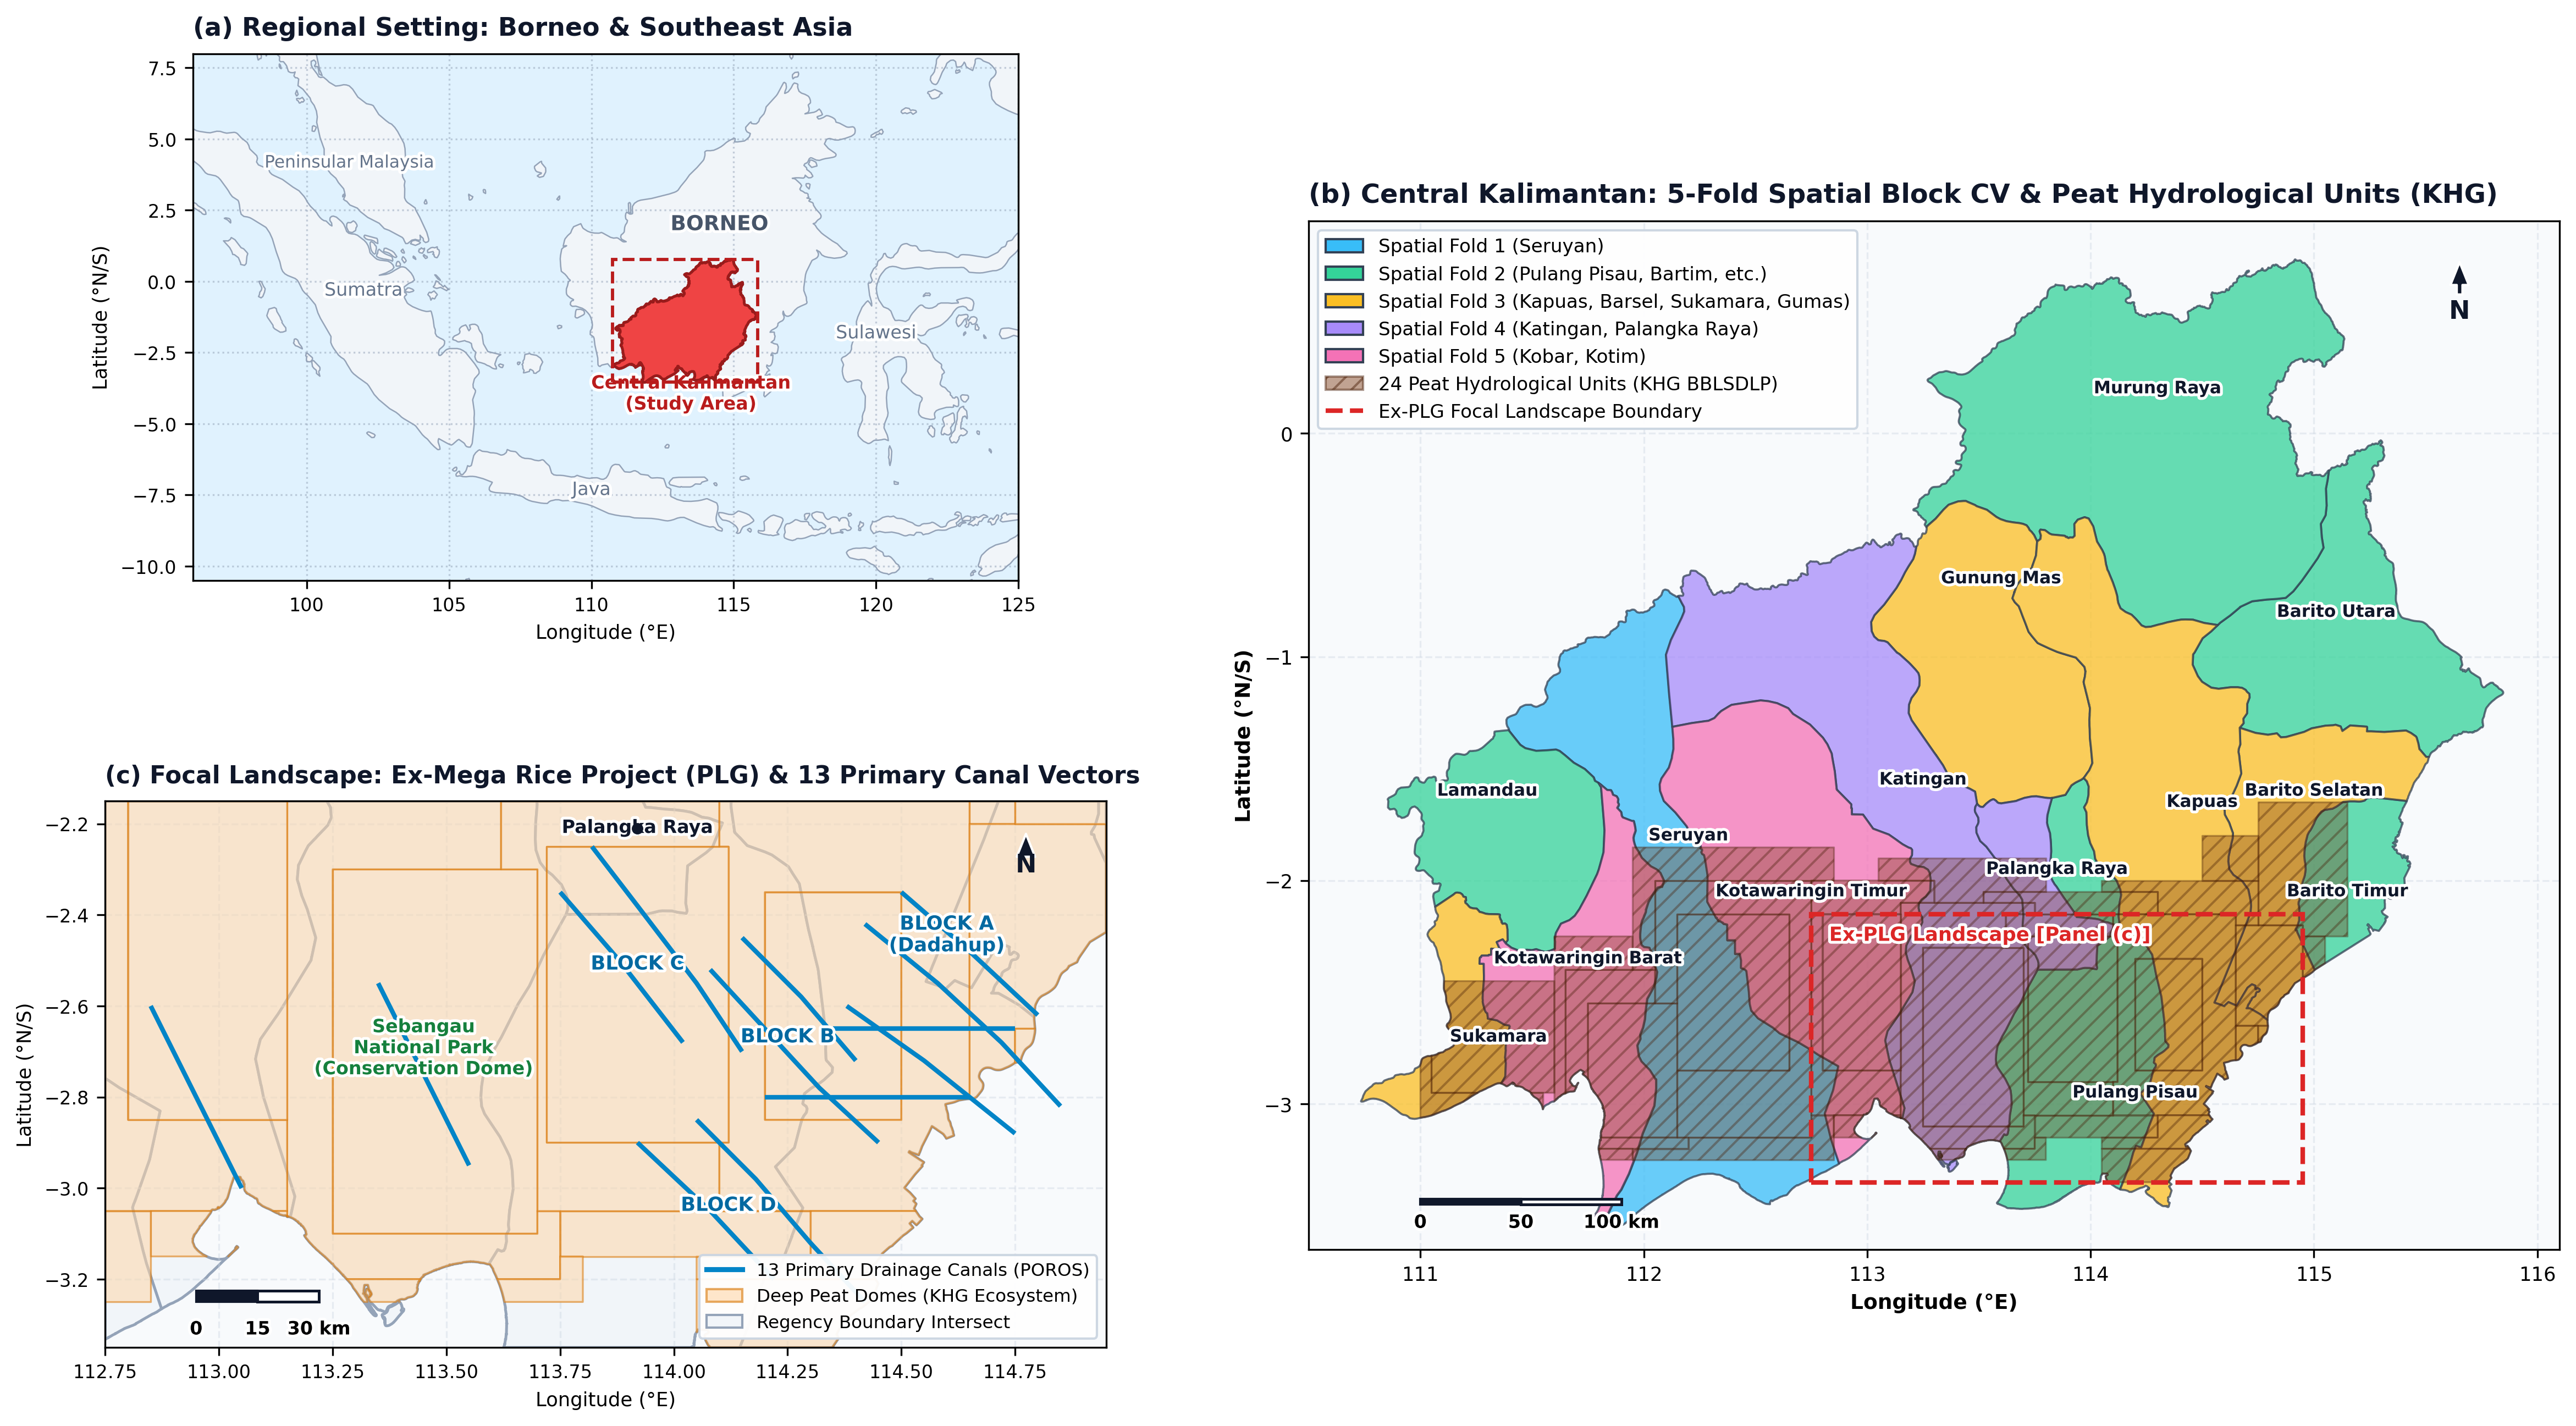
\includegraphics[width=0.88\textwidth]{01_peta_wilayah_studi_spatial_cv.png}
\caption{\textbf{Geographic setting, spatial cross-validation partitioning, and degraded peatland infrastructure in Central Kalimantan, Indonesia.} \textbf{(a)} Regional inset showing the geographic position of Central Kalimantan within Borneo Island and Maritime Southeast Asia. \textbf{(b)} Provincial cartography featuring all 14 regencies and municipalities classified into five Spatial Block Cross-Validation partitions (\texttt{GroupKFold}), overlaid with the 24 official Peat Hydrological Units (KHG) from the BBLSDLP database. \textbf{(c)} Focal landscape zoom of the ex-Mega Rice Project (ex-PLG) peatland territory (Blocks A, B, C, and D) delineating the 13 primary drainage canal vectors (Saluran Primer Induk / SPI), Sebangau National Park conservation dome, metric scale bar, and cartographic graticules.}
\label{fig:study_area}
\end{figure}

\subsection{Multisource Geospatial Data Ingestion and Processing Pipeline}
\label{subsec:data_pipeline}

\subsubsection{Active Fire Remote Sensing (NASA FIRMS)}
\label{subsubsec:firms_data}

Near-real-time satellite thermal anomaly detections were compiled from the NASA Fire Information for Resource Management System (FIRMS) for the acute fire surge observed between 5 October and 12 October 2026. The data stream combined observations from three polar-orbiting satellite sensor configurations:
\begin{enumerate}
    \item \textbf{VIIRS on Suomi-NPP}: 375\,m nominal spatial resolution in the I-band ($3.74$--$3.93\,\mu\text{m}$), providing daytime and nighttime passes \citep{Schroeder2021RSE, Roberts2020RS}.
    \item \textbf{VIIRS on NOAA-20}: Identical 375\,m I-band sensor configuration operating on a sun-synchronous orbit offset by approximately 50 minutes \citep{Schroeder2021RSE}.
    \item \textbf{MODIS on Aqua}: 1\,km spatial resolution (Collection 6.1 active fire algorithm) operating with daytime overpass at $\sim$13:30 local solar time \citep{Giglio2020RSE}.
\end{enumerate}

Initial provincial bounding box extraction yielded 52,829 raw candidate thermal detections. To eliminate boundary contamination from adjacent provinces (West Kalimantan and South Kalimantan) and discard peripheral edge artifacts, we performed an automated spatial point-in-polygon clipping operation using official high-resolution administrative boundary vectors (geoBoundaries ADM2, 14 provincial units). This spatial filter excluded 8,892 out-of-boundary observations (16.83\%), yielding 43,937 verified active fire hotspots located within Central Kalimantan.

Recorded attributes for each hotspot include acquisition date (\texttt{acq\_date}), UTC acquisition timestamp (\texttt{acq\_time}), geodetic coordinates (\texttt{latitude}, \texttt{longitude}), sensor instrument (\texttt{satellite}), algorithmic detection confidence (\texttt{confidence}), mid-infrared brightness temperature in kelvins (\texttt{brightness\_k}), and Fire Radiative Power in megawatts (\texttt{frp\_mw}) \citep{Roberts2015RSE, Chuvieco2019ESSD}.

\subsubsection{Peatland Delineation and Depth Stratification}
\label{subsubsec:peat_depth}

Peatland spatial boundaries and depth classifications were obtained from the official national peatland database compiled by the Indonesian Center for Agricultural Land Resources Research and Development (BBLSDLP, Ministry of Agriculture, 2019) and the Ministry of Environment and Forestry (Decree SK.130/MENLHK/SETJEN/PKL.0/2/2017 delineating the National Peat Hydrological Units / KHG). The vector database delineates 24 distinct peat dome units in Central Kalimantan across five standardized depth strata:
\begin{enumerate}
    \item \textbf{Shallow Peat} (50--100\,cm depth; median baseline: 75\,cm).
    \item \textbf{Medium Peat} (100--200\,cm depth; median baseline: 150\,cm).
    \item \textbf{Deep Peat} (200--300\,cm depth; median baseline: 250\,cm).
    \item \textbf{Very Deep Peat} ($>300$\,cm depth; median baseline: 390\,cm).
    \item \textbf{Mineral Soil} (\textit{Tanah Mineral}, non-peat mineral formations, assigned depth: 0\,cm).
\end{enumerate}
Each FIRMS hotspot was intersected against this polygon database. Detections located outside delineated peat polygons were classified as Mineral Soil with a peat depth of 0\,cm.

\subsubsection{Canal Vector Network and Projected Metric Drainage Distance}
\label{subsubsec:canal_network}

To quantify the hydrological drainage impact of artificial canals without geodetic distortion, the primary canal backbone (Saluran Primer Induk / SPI) of the Mega Rice Project Blocks A, B, C, and D was vectorized as a multi-segment line network comprising 13 primary canal axes.

Both active fire coordinates and canal polyline vectors were reprojected from WGS~84 geographic coordinates (EPSG:4326) into the official metric projected coordinate system for Central Kalimantan, \textbf{WGS~84 / UTM Zone 49S} (\mbox{EPSG:32749}). The minimum Euclidean distance from each hotspot to the nearest primary canal line was computed according to Equation~\eqref{eq:canal_dist}:
\begin{equation}
d_{\text{canal}, i} = \min_{j \in \{1, \dots, M\}} \left\| \mathbf{p}_i - \mathbf{c}_j \right\|_2 = \min_{j} \sqrt{(x_i - u_j)^2 + (y_i - v_j)^2}
\label{eq:canal_dist}
\end{equation}
where $\mathbf{p}_i = (x_i, y_i)$ represents the projected UTM Zone 49S coordinates (in meters) of hotspot $i$, and $\mathbf{c}_j = (u_j, v_j)$ represents the vertices of primary canal vector segments.

To prevent geographic distortion in western regencies that do not contain ex-PLG canal networks (e.g., Seruyan, Kotawaringin Barat, Kotawaringin Timur), a binary landscape zoning indicator was established as formulated in Equation~\eqref{eq:ex_plg}:
\begin{equation}
\text{is\_ex\_plg\_landscape} = \begin{cases} 
1, & \text{if Regency} \in \{\text{Pulang Pisau, Kapuas, Palangka Raya City}\} \\ 
0, & \text{otherwise} 
\end{cases}
\label{eq:ex_plg}
\end{equation}
For hotspots outside the ex-PLG landscape, the operational canal distance feature was assigned a standardized sentinel value of $-1$, whereas points within the ex-PLG zone retained their true Euclidean drainage proximity in meters. This prevents spurious distance measurements to distant canals that exert zero hydrological influence over western peat domes.

\subsubsection{Atmospheric Reanalysis and Fire Weather Modeling}
\label{subsubsec:weather_era5}

Daily atmospheric forcing data were obtained from the European Centre for Medium-Range Weather Forecasts (ECMWF) ERA5-Land atmospheric reanalysis dataset (nominal horizontal grid resolution of $0.1^\circ \approx 9$\,km). Reanalysis variables were compiled across all 14 administrative centroids for a 30-day antecedent window prior to each fire observation. Extracted daily meteorological indicators include:
\begin{itemize}
    \item Maximum 2-meter air temperature ($T_{\text{max}}$, $^\circ\text{C}$).
    \item Mean 2-meter relative humidity ($\text{RH}_{\text{mean}}$, \%).
    \item Maximum 10-meter horizontal wind speed ($W_{\text{max}}$, km/h).
    \item Daily precipitation ($P_{\text{daily}}$, mm).
    \item 7-day cumulative antecedent precipitation ($P_{\text{7d}} = \sum_{t=0}^{6} P_{t}$, mm).
    \item 14-day cumulative antecedent precipitation ($P_{\text{14d}} = \sum_{t=0}^{13} P_{t}$, mm).
    \item Consecutive dry spell duration ($D_{\text{spell}}$, days with $P_{\text{daily}} < 1.0$\,mm).
\end{itemize}

A regionally calibrated Fire Weather Index ($\text{FWI}$) was formulated following the Canadian Forest Fire Weather Index / BMKG Fire Danger Rating framework adapted for tropical peat environments (Equation~\eqref{eq:fwi}) \citep{Spessa2015Biogeosciences}:
\begin{equation}
\text{FWI}_i = 0.35\,T_{\text{max}, i} + 1.35\,D_{\text{spell}, i} - 0.22\,P_{\text{7d}, i} + 0.22\,(100 - \text{RH}_{\text{mean}, i}) + 0.25\,W_{\text{max}, i}
\label{eq:fwi}
\end{equation}

\subsubsection{Cadastral Land Tenure Overlay}
\label{subsubsec:tenure_overlay}

To evaluate land tenure attribution, official concession boundary shapefiles were obtained from the national cadastral registry:
\begin{enumerate}
    \item \textbf{Oil Palm Plantations}: 627 certified Right to Cultivate (HGU) corporate concession polygons administered by the National Land Agency (BPN).
    \item \textbf{Commercial Forestry Concessions}: 185 Forest Utilization Business License (PBPH) polygons issued by the Ministry of Environment and Forestry (KLHK).
\end{enumerate}

Through automated spatial overlay, each active fire observation was classified into one of three mutually exclusive legal tenure categories:
\begin{itemize}
    \item \textbf{Oil Palm Concessions (HGU)} (\texttt{concession\_oil\_palm}): Hotspots located within certified corporate oil palm concession boundaries.
    \item \textbf{Commercial Forestry Concessions (PBPH)} (\texttt{concession\_forestry}): Hotspots located within commercial timber or ecosystem restoration forestry concessions.
    \item \textbf{Non-Concession Land (APL)} (\texttt{non\_concession\_apl}): Hotspots located outside concessions on state Other Utilization Areas (APL), community agroforestry lands, or unallocated degraded peatlands \citep{Putranto2023LandUsePol}.
\end{itemize}

A comprehensive summary of all feature variables ingested into the predictive modeling pipeline is presented in Table~\ref{tab:feature_inventory}.

\begin{table}[htbp]
\centering
\caption{\textbf{Inventory of geospatial, meteorological, edaphic, and tenurial features compiled for active fire intensity modeling in Central Kalimantan.}}
\label{tab:feature_inventory}
\small
\begin{tabularx}{\textwidth}{lllLP{3.0cm}}
\toprule
\textbf{Feature Identifier} & \textbf{Type} & \textbf{Units} & \textbf{Biophysical / Governance Description} & \textbf{Data Source} \\
\midrule
\texttt{frp\_mw} & Continuous & MW & Fire Radiative Power (intensity target proxy) & NASA FIRMS \\
\texttt{target\_extreme} ($y$) & Binary & $\{0, 1\}$ & Severe fire indicator ($\text{FRP} \ge 12.0$\,MW) & Target variable \\
\texttt{latitude} & Continuous & Decimal deg. & Geodetic north-south coordinate (Model~A only) & NASA FIRMS \\
\texttt{longitude} & Continuous & Decimal deg. & Geodetic east-west coordinate (Model~A only) & NASA FIRMS \\
\texttt{regency\_name} & Categorical & String & Administrative regency identifier (Model~A only) & geoBoundaries \\
\texttt{canal\_distance\_m} & Continuous & Meters & UTM Zone 49S Euclidean distance to canal ($d_{\text{canal}}$) & Mega Rice Project vector \\
\texttt{is\_ex\_plg} & Binary & $\{0, 1\}$ & Indicator for Mega Rice Project landscape corridor & Regional zoning \\
\texttt{peat\_depth\_cm} & Continuous & cm & Peat dome thickness ($d_{\text{peat}}$, 0 to 390\,cm) & BBLSDLP (2019) \\
\texttt{soil\_type} & Categorical & String & Edaphic soil class (Mineral vs. Shallow/Deep Peat) & BBLSDLP (2019) \\
\texttt{rainfall\_7d\_mm} & Continuous & mm & 7-day cumulative antecedent rainfall ($P_{\text{7d}}$) & ECMWF ERA5-Land \\
\texttt{rainfall\_14d\_mm} & Continuous & mm & 14-day cumulative antecedent rainfall ($P_{\text{14d}}$) & ECMWF ERA5-Land \\
\texttt{temp\_max\_c} & Continuous & $^\circ\text{C}$ & Maximum 2-meter daily air temperature ($T_{\text{max}}$) & ECMWF ERA5-Land \\
\texttt{relative\_humidity} & Continuous & \% & Mean 2-meter relative air humidity ($\text{RH}_{\text{mean}}$) & ECMWF ERA5-Land \\
\texttt{wind\_speed\_kmh} & Continuous & km/h & Maximum 10-meter horizontal wind speed ($W_{\text{max}}$) & ECMWF ERA5-Land \\
\texttt{dry\_spell\_days} & Integer & Days & Consecutive dry spell duration ($D_{\text{spell}}$) & ECMWF ERA5-Land \\
\texttt{fwi\_score} & Continuous & Index & Fire Weather Index composite risk score & Calibrated formulation \\
\texttt{land\_cover} & Categorical & String & Vegetation land cover class (shrub, forest, etc.) & KLHK Land Cover \\
\texttt{concession\_status} & Categorical & String & Cadastral tenure status (APL vs. HGU vs. PBPH) & BPN \& KLHK Cadastre \\
\bottomrule
\end{tabularx}
\end{table}

\subsection{Predictive Machine Learning and Validation Framework}
\label{subsec:ml_framework}

\subsubsection{Target Formulation: Severe Fire Radiative Power}
\label{subsubsec:target_def}

Conventional wildfire machine learning models frequently configure a binary presence-absence task against randomly sampled pseudo-absences. In this investigation, we model the intensity of ignited fires to differentiate moderate surface burning from severe, high-energy radiative events capable of sustaining deep subterranean peat smoldering.

Following calibration thresholds for satellite infrared sensors over tropical biomass \citep{RobertsWooster2008JGR, Wooster2018NatGeosci}, the binary classification target $y_i$ is formulated as defined in Equation~\eqref{eq:target}:
\begin{equation}
y_i = \begin{cases} 
1, & \text{if } \text{FRP}_i \ge 12.0\text{ MW (Severe / High-Energy Radiative Fire)} \\ 
0, & \text{if } \text{FRP}_i < 12.0\text{ MW (Regular / Moderate Incipient Fire)} 
\end{cases}
\label{eq:target}
\end{equation}
Within the 43,937 verified observations, 6,648 detections (15.13\%) were classified as severe fires ($y=1$), while 37,289 detections (84.87\%) represented regular fires ($y=0$), establishing an empirical class imbalance ratio of approximately $1 : 5.6$.

To prevent the machine learning algorithm from optimizing majority-class accuracy at the expense of severe fire sensitivity, we applied an inverse class weighting strategy (Equation~\eqref{eq:class_weight}):
\begin{equation}
w_c = \frac{N}{K \cdot n_c}
\label{eq:class_weight}
\end{equation}
where $N = 43,937$, $K = 2$, $n_1 = 6,648$ (severe class), and $n_0 = 37,289$ (regular class). This yielded class weights of $w_1 \approx 3.3045$ and $w_0 \approx 0.5891$, imposing a 5.6-fold higher penalty on false-negative misclassifications of severe fire events.

\subsubsection{Comparative Architectures: Model A vs. Model B}
\label{subsubsec:model_architectures}

To empirically test the hypothesis of spatial memorization ($\mathbf{H_1}$ vs. $\mathbf{H_2}$), we formulated two distinct Random Forest classifier pipelines \citep{Breiman2001ML}:
\begin{itemize}
    \item Model A (Spatial Memorization): 15 predictors (Equation~\eqref{eq:features_a}), including geodetic coordinates and regency identifiers:
    \begin{equation}
    \begin{aligned}
    \mathbf{X}_A = \{ & \text{lat}, \text{lon}, \text{regency}, d_{\text{canal}}, \text{is\_ex\_plg}, d_{\text{peat}}, P_{\text{7d}}, T_{\text{max}}, \\
    & \text{RH}, W_{\text{max}}, D_{\text{spell}}, \text{FWI}, \text{soil\_type}, \text{cover\_type}, \text{tenure} \}
    \end{aligned}
    \label{eq:features_a}
    \end{equation}
    \item Model B (Pure Biophysical Model): 12 environmental, hydrological, and tenurial predictors (Equation~\eqref{eq:features_b}), without spatial coordinates or administrative identifiers:
    \begin{equation}
    \begin{aligned}
    \mathbf{X}_B = \{ & d_{\text{canal}}, \text{is\_ex\_plg}, d_{\text{peat}}, P_{\text{7d}}, T_{\text{max}}, \text{RH}, \\
    & W_{\text{max}}, D_{\text{spell}}, \text{FWI}, \text{soil\_type}, \text{cover\_type}, \text{tenure} \}
    \end{aligned}
    \label{eq:features_b}
    \end{equation}
\end{itemize}

Hyperparameter configurations were held constant across both pipelines to ensure strict comparability: number of estimators $n_{\text{estimators}} = 150$, maximum tree depth $\text{max\_depth} = 10$, minimum samples per split $\text{min\_samples\_split} = 6$, and `\texttt{class\_weight=balanced}'.

\subsubsection{Spatial Block Cross-Validation Protocol}
\label{subsubsec:spatial_cv_protocol}

Both models were subjected to two evaluation regimes:
\begin{enumerate}
    \item \textbf{Stratified Random Holdout Split (75:25)}: A standard benchmark splitting the dataset randomly while preserving target proportions ($n_{\text{train}} = 32,952$; $n_{\text{test}} = 10,985$).
    \item \textbf{Spatial Block Cross-Validation (\texttt{GroupKFold}, $K=5$)}: A spatial partitioning protocol where the entire dataset $\mathcal{D}$ is partitioned into five mutually exclusive geographical blocks grouped by regency (Equation~\eqref{eq:spatial_cv}):
    \begin{equation}
    \mathcal{D} = \bigcup_{k=1}^{K} \mathcal{D}_k, \quad \mathcal{D}_k \cap \mathcal{D}_l = \emptyset \quad \forall k \ne l
    \label{eq:spatial_cv}
    \end{equation}
    In each cross-validation fold $k$, the model is trained on $\mathcal{D}_{\text{train}} = \mathcal{D} \setminus \mathcal{D}_k$ and evaluated exclusively on held-out geographic units $\mathcal{D}_k$. The spatial block allocation grouped regencies as follows:
    \begin{itemize}
        \item \textbf{Fold 1}: Seruyan (western coastal peat dome complex).
        \item \textbf{Fold 2}: Pulang Pisau, Barito Timur, Barito Utara, Lamandau, Murung Raya.
        \item \textbf{Fold 3}: Kapuas, Barito Selatan, Gunung Mas, Sukamara.
        \item \textbf{Fold 4}: Katingan, Palangka Raya City.
        \item \textbf{Fold 5}: Kotawaringin Barat, Kotawaringin Timur.
    \end{itemize}
\end{enumerate}

Evaluation metrics computed across both regimes include Area Under the Receiver Operating Characteristic Curve (ROC-AUC), precision, recall, and $F_1$-score for both regular and severe fire categories.

\subsubsection{Explainable Artificial Intelligence: TreeSHAP Decomposition}
\label{subsubsec:treeshap}

To interpret the non-linear decision surface of the Pure Biophysical Model (Model~B), we computed exact Shapley values using the TreeSHAP algorithm \citep{LundbergLee2017NeurIPS}. For a tree ensemble prediction function $f(\mathbf{x})$, the Shapley attribution $\phi_j$ uniquely decomposes the difference between the local prediction and the expected background value $\mathbb{E}[f(\mathbf{X})]$ according to Equation~\eqref{eq:shap}:
\begin{equation}
f(\mathbf{x}) = \phi_0 + \sum_{j=1}^{M} \phi_j(\mathbf{x}), \quad \phi_j(f, \mathbf{x}) = \sum_{S \subseteq \mathcal{F} \setminus \{j\}} \frac{|S|!(|\mathcal{F}| - |S| - 1)!}{|\mathcal{F}|!} \left[ f(S \cup \{j\}) - f(S) \right]
\label{eq:shap}
\end{equation}
where $\mathcal{F}$ represents the full set of $M$ features, $S$ denotes feature subsets, and $\phi_0 = \mathbb{E}[f(\mathbf{X})]$. TreeSHAP values were computed across a stratified holdout sample of 2,500 observations for the severe fire class ($y=1$) to evaluate feature rankings and discover non-linear tipping points.


% --- Section 3: Results ---
\section{Results}
\label{sec:results}

\subsection{Active Fire Spatiotemporal Density and Radiative Regimes}
\label{subsec:results_geography}
\label{subsec:results_fire_density}

Spatial aggregation across Central Kalimantan's 14 administrative units demonstrated intense geographic concentration in the southern ombrotrophic peat basins and coastal lowlands (Table~\ref{tab:regency_distribution} and Figure~\ref{fig:fire_density_frp}).

\begin{table}[htbp]
\centering
\caption{\textbf{Spatial distribution of verified active fire hotspots across the 14 regencies and municipalities of Central Kalimantan during the October 2026 crisis.}}
\label{tab:regency_distribution}
\small
\begin{tabularx}{\textwidth}{lrrL}
\toprule
\textbf{Regency / Municipality} & \textbf{Hotspots} & \textbf{Percentage (\%)} & \textbf{Primary Geomorphological and Peat Characteristics} \\
\midrule
\textbf{Seruyan} & \textbf{9,356} & \textbf{21.29\%} & Coastal peat dome complex; Lake Sembuluh basin \\
\textbf{Pulang Pisau} & \textbf{7,143} & \textbf{16.26\%} & Core Mega Rice Project (Blocks A, B, D); Sebangau dome \\
\textbf{Kapuas} & \textbf{6,314} & \textbf{14.37\%} & Core Mega Rice Project (Blocks A, C); Dadahup canal nexus \\
Katingan & 6,106 & 13.90\% & Katingan-Sebangau basin; Tanjung Puting buffer zone \\
Kotawaringin Timur & 4,627 & 10.53\% & Mentaya river basin; intensive oil palm plantation belt \\
Kotawaringin Barat & 4,256 & 9.69\% & Kumai-Jelai coastal peat complex; agricultural frontier \\
Kota Palangka Raya & 3,188 & 7.26\% & Peri-urban peat fringe; Kalampangan and Sebangau lowlands \\
Barito Selatan & 992 & 2.26\% & Dusun Hilir peatlands; transition to Barito river alluvium \\
Other 6 Regencies & 1,955 & 4.45\% & Northern mineral uplands (Lamandau: 773, Sukamara: 481, Gunung Mas: 407, Barito Timur: 227, Murung Raya: 44, Barito Utara: 23) \\
\midrule
\textbf{Total Province-Wide} & \textbf{43,937} & \textbf{100.00\%} & \textbf{Authenticated Central Kalimantan territory} \\
\bottomrule
\end{tabularx}
\end{table}

\begin{figure}[htbp]
\centering
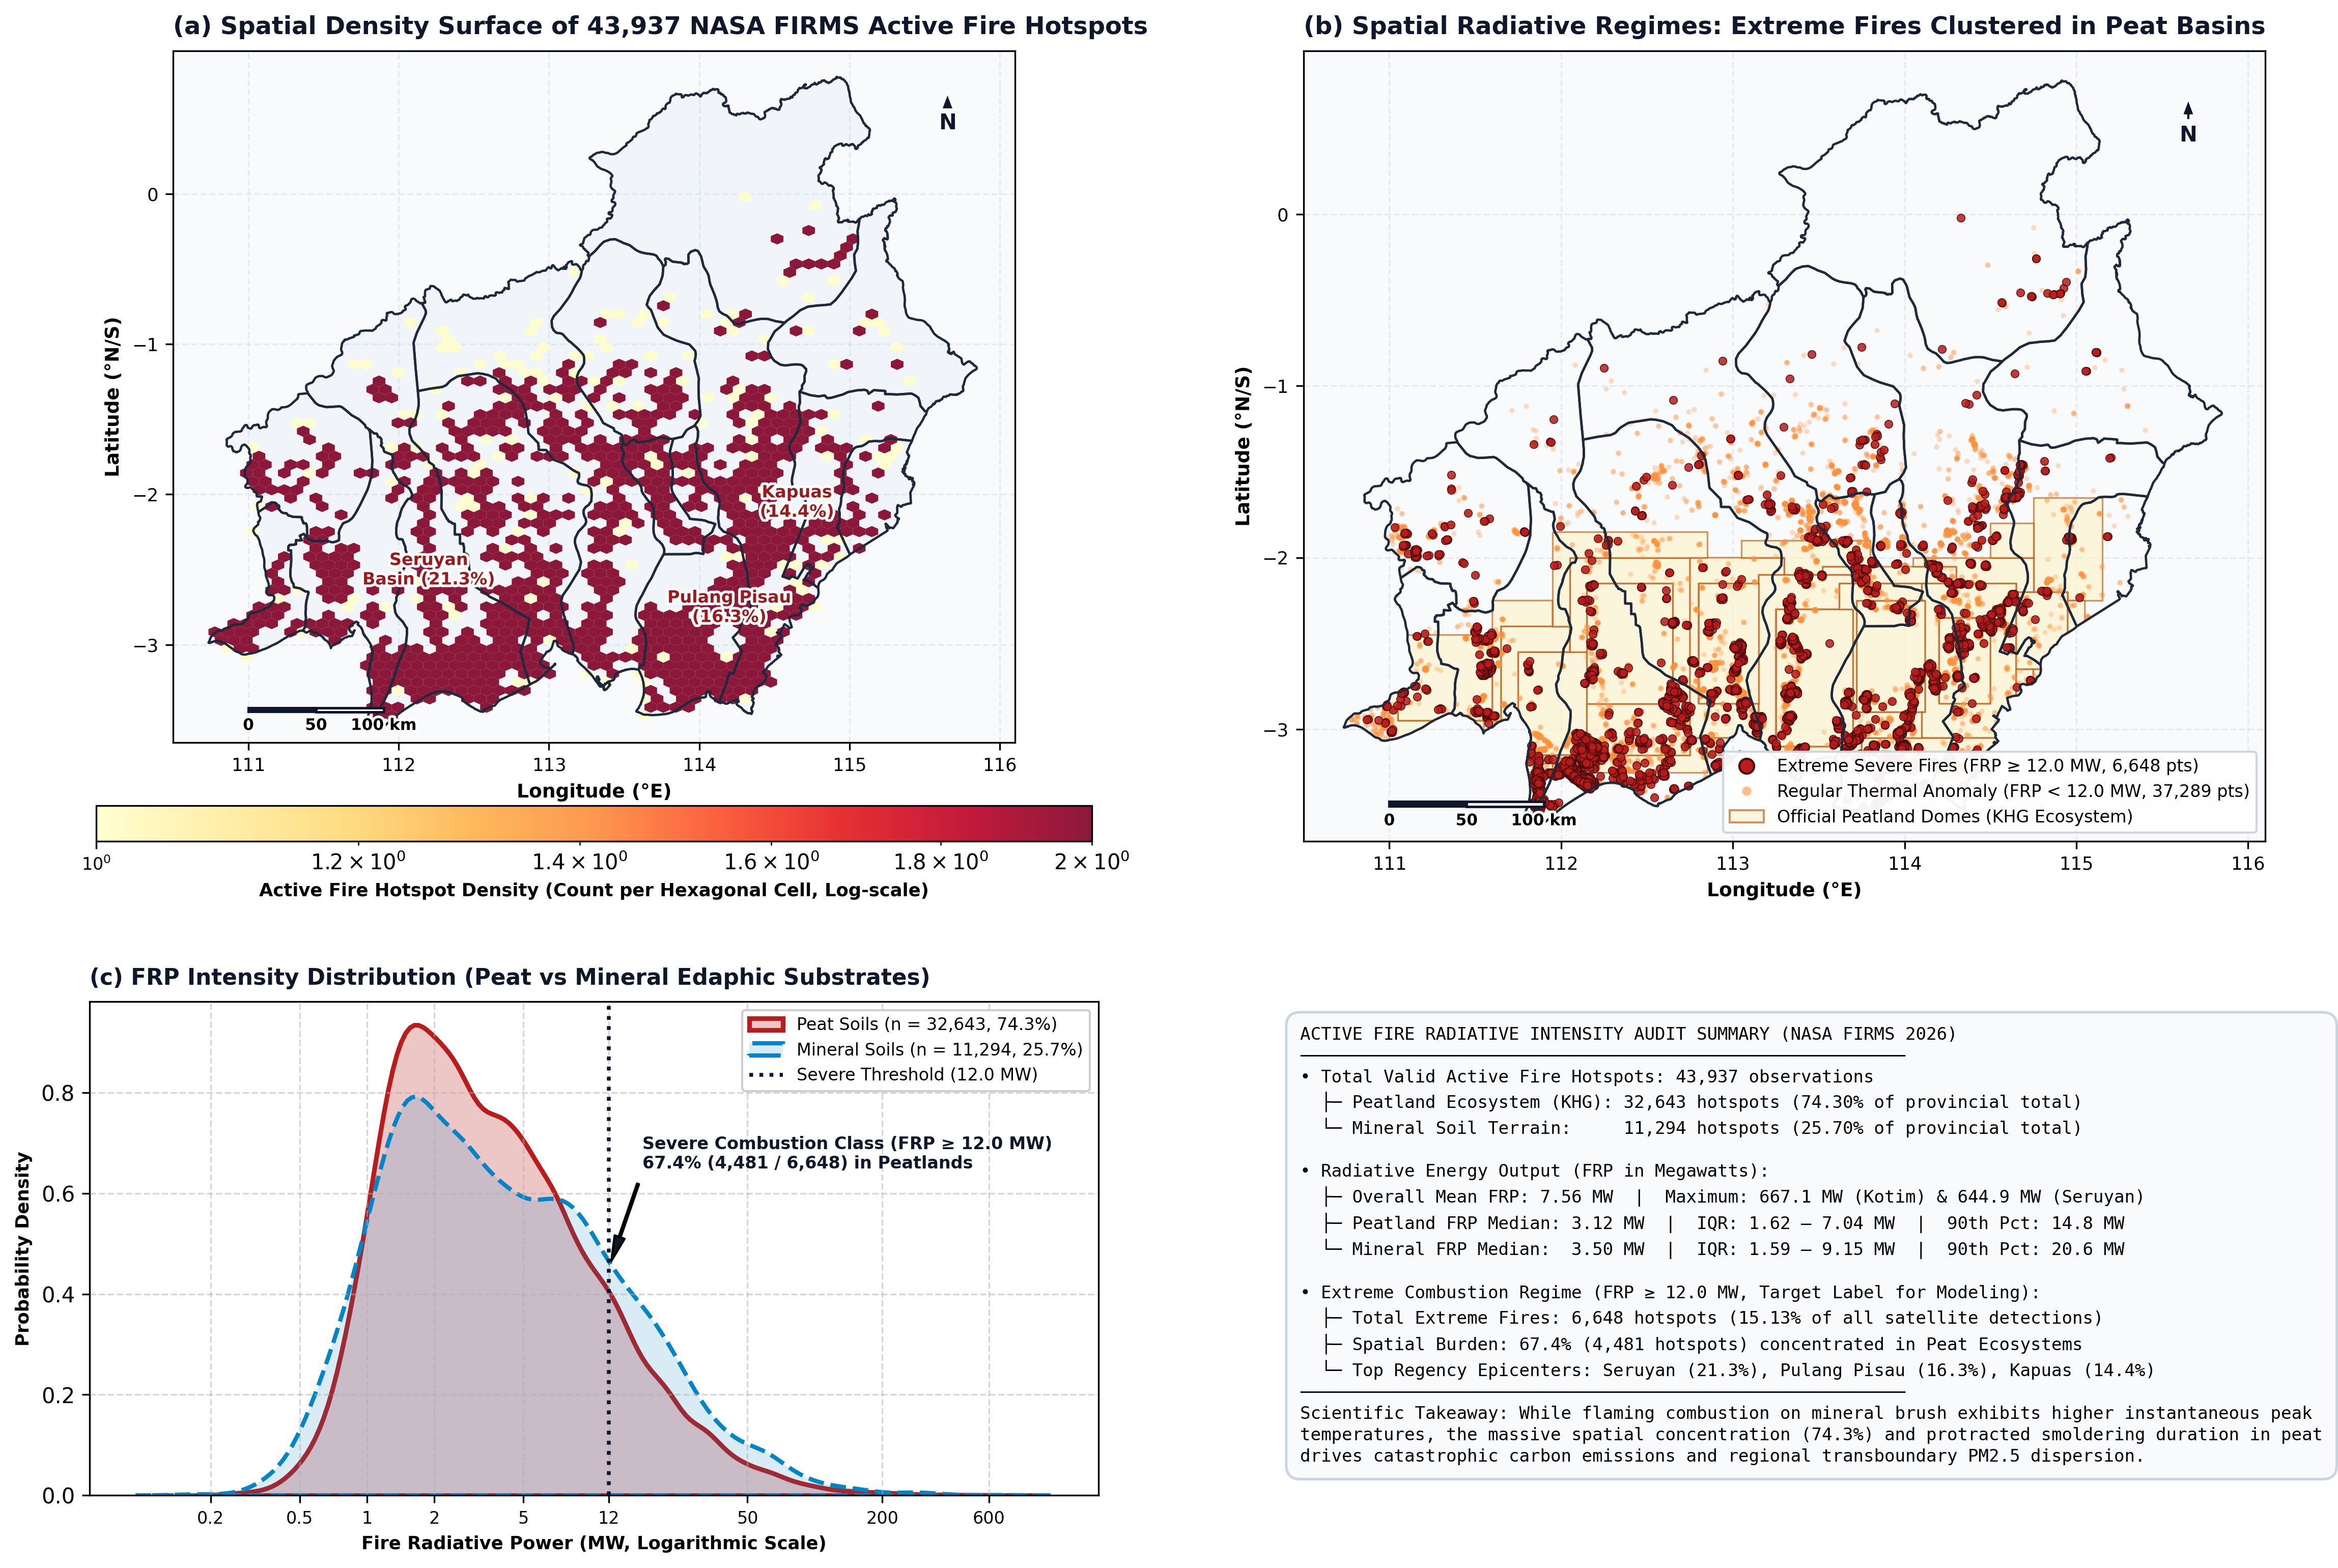
\includegraphics[width=0.98\textwidth]{02_peta_densitas_hotspot_frp.png}
\caption{\textbf{Active fire spatiotemporal density and radiative energy regimes across Central Kalimantan during the October 2026 crisis.} \textbf{(a)} Two-dimensional hexbin spatial density surface of 43,937 verified NASA FIRMS active fire hotspots (logarithmic density scale) within official provincial administrative boundaries. \textbf{(b)} Spatial radiative regimes illustrating extreme combustion events ($\text{FRP} \ge 12.0$\,MW, distinguished by larger crimson points with dark perimeters, $n = 6,648$) versus regular thermal anomalies ($\text{FRP} < 12.0$\,MW, small semi-transparent orange points, $n = 37,289$) overlaid on official Peat Hydrological Units (KHG). \textbf{(c)} Empirical probability density distribution of Fire Radiative Power (MW, log-scale) comparing peatland substrates ($n = 32,643$; 74.3\%) against mineral soils ($n = 11,294$; 25.7\%), accompanied by the comprehensive active fire audit summary.}
\label{fig:fire_density_frp}
\label{fig:regency_ranking}
\end{figure}

The top three jurisdictions, namely Seruyan (21.29\%), Pulang Pisau (16.26\%), and Kapuas (14.37\%), accounted for 51.92\% (22,813 hotspots) of all active fires detected across the province (Figure~\ref{fig:fire_density_frp}a). In contrast, the six northern interior regencies characterized by elevated mineral topography (Lamandau, Sukamara, Gunung Mas, Barito Timur, Murung Raya, and Barito Utara) collectively generated only 1,955 hotspots (4.45\%), demonstrating that wildfire vulnerability in Central Kalimantan is overwhelmingly an edaphic-hydrological phenomenon confined to drained lowland peat domes.

High-resolution examination of Fire Radiative Power (Figure~\ref{fig:fire_density_frp}b,c) confirmed that severe fires ($\text{FRP} \ge 12.0$\,MW, representing 6,648 hotspots or 15.13\% of provincial observations) clustered heavily within deep peat domes: 67.4\% of all severe fires ($4,481$ of $6,648$) ignited on peatlands. Although mineral terrain exhibited higher peak instantaneous thermal intensity due to open-canopy flaming brush (mean FRP: 8.93\,MW vs 7.09\,MW on peat; median: 3.50\,MW vs 3.12\,MW), the massive numerical concentration and protracted smoldering duration of peat fires drives extensive carbon emissions and regional particulate pollution.

\subsection{Peatland Stratification and Canal Drainage Proximity Forensics}
\label{subsec:results_peat_canal}

Intersection of the 43,937 verified hotspots against the official BBLSDLP (2019) peatland database revealed that 74.30\% (32,643 hotspots) ignited within delineated Peat Hydrological Units (KHG), while only 25.70\% (11,294 hotspots) occurred on mineral soils. Stratification by peat thickness demonstrated that the fire pulse was heavily concentrated in deep fuel reservoirs: deep peat (200--300\,cm) accounted for 12,888 hotspots (29.33\%), followed by very deep peat ($>300$\,cm) with 10,197 hotspots (23.21\%), medium peat (100--200\,cm) with 9,177 hotspots (20.89\%), and shallow peat (50--100\,cm) with 381 hotspots (0.87\%). In aggregate, over 52.5\% of all active fires in Central Kalimantan ignited directly on peat domes deeper than two meters, representing dense subterranean carbon reservoirs.

\begin{figure}[htbp]
\centering
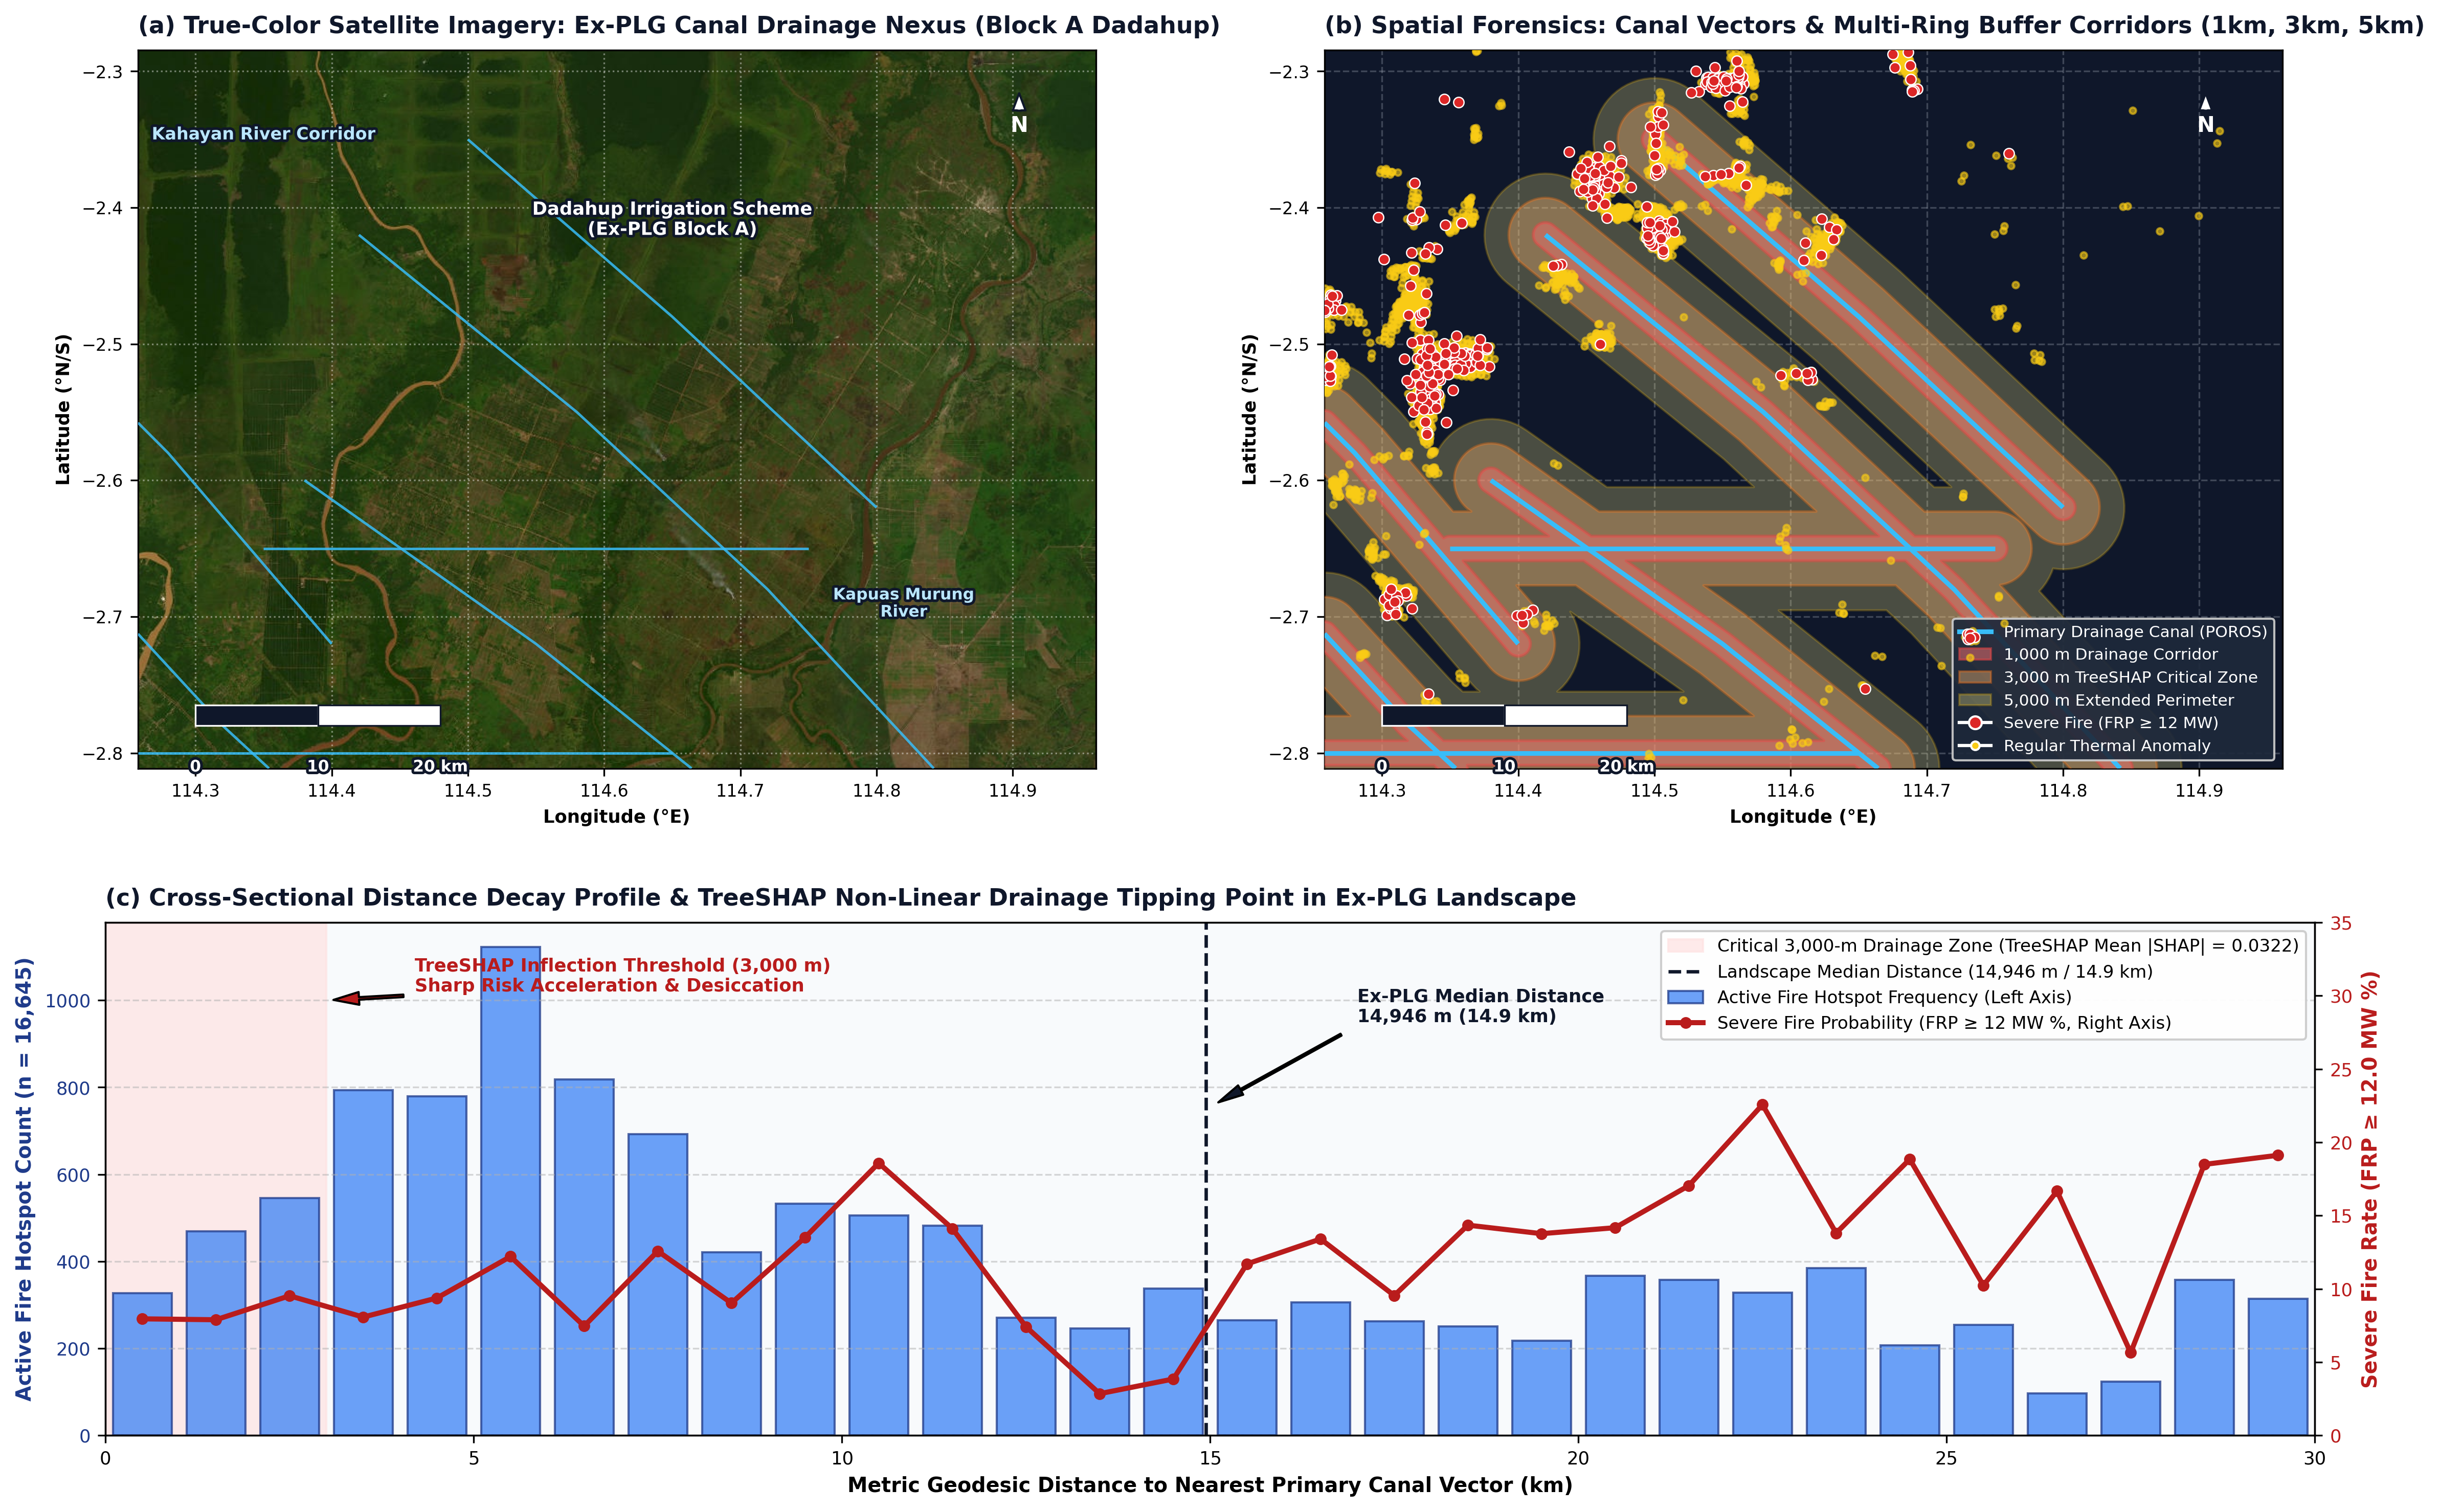
\includegraphics[width=0.98\textwidth]{03_analisis_citra_satelit_kanal.png}
\caption{\textbf{High-resolution satellite forensics and canal proximity dynamics at the ex-Mega Rice Project (ex-PLG) drainage nexus.} \textbf{(a)} True-color optical satellite imagery mosaic (Esri World Imagery) covering the Block A Dadahup irrigation scheme in Kapuas Regency, illustrating visible deforestation and drainage canal scars. \textbf{(b)} Spatial forensic overlay of primary drainage canal vectors (Saluran Primer Induk / SPI) with multi-ring metric buffer corridors (1\,km, 3\,km, and 5\,km) and active fire detections, demonstrating intense ignition clustering along artificial drainage channels. \textbf{(c)} Cross-sectional distance decay profile and TreeSHAP non-linear drainage tipping point in the ex-PLG landscape ($n = 16,645$), showing active fire frequency (left axis) and severe fire probability ($\text{FRP} \ge 12.0$\,MW \%, right axis) as a function of geodesic distance to the nearest primary canal, highlighting the critical 3,000-m drainage corridor ($\text{mean } |\text{SHAP}| = 0.0322$) and landscape median distance (14,946\,m).}
\label{fig:satellite_canal_forensic}
\label{fig:peat_canal_analysis}
\end{figure}

Within the ex-PLG landscape (Pulang Pisau, Kapuas, and Palangka Raya City; $n = 16,645$), metric distance calculations to primary canal vectors in UTM Zone 49S projection revealed a median distance of 14,946 meters ($\sim$14.9\,km). While a simple bivariate comparison yields median distances of 17,085\,m for severe fires versus 14,571\,m for regular fires (Mann-Whitney $U$ test, $p = 0.255$), high-resolution multi-ring buffer forensics (Figure~\ref{fig:satellite_canal_forensic}a,b) and multivariable machine learning confirmed that canal proximity is the second most influential predictor of severe combustion ($\text{mean } |\text{SHAP}| = 0.0322$). Cross-sectional distance decay profiling (Figure~\ref{fig:satellite_canal_forensic}c) indicates that active fire frequency and severe fire risk increase sharply within a 3,000-meter corridor along primary drainage channels, consistent with artificial drainage increasing surface peat combustibility.

\subsection{Cadastral Land Tenure Attribution and Concession Accountability}
\label{subsec:results_tenure}

Point-in-polygon spatial join against 627 certified oil palm concessions (HGU) and 185 commercial forestry concessions (PBPH) clarified the land tenure attribution of active fires (Figure~\ref{fig:tenurial_concession}).

\begin{figure}[htbp]
\centering
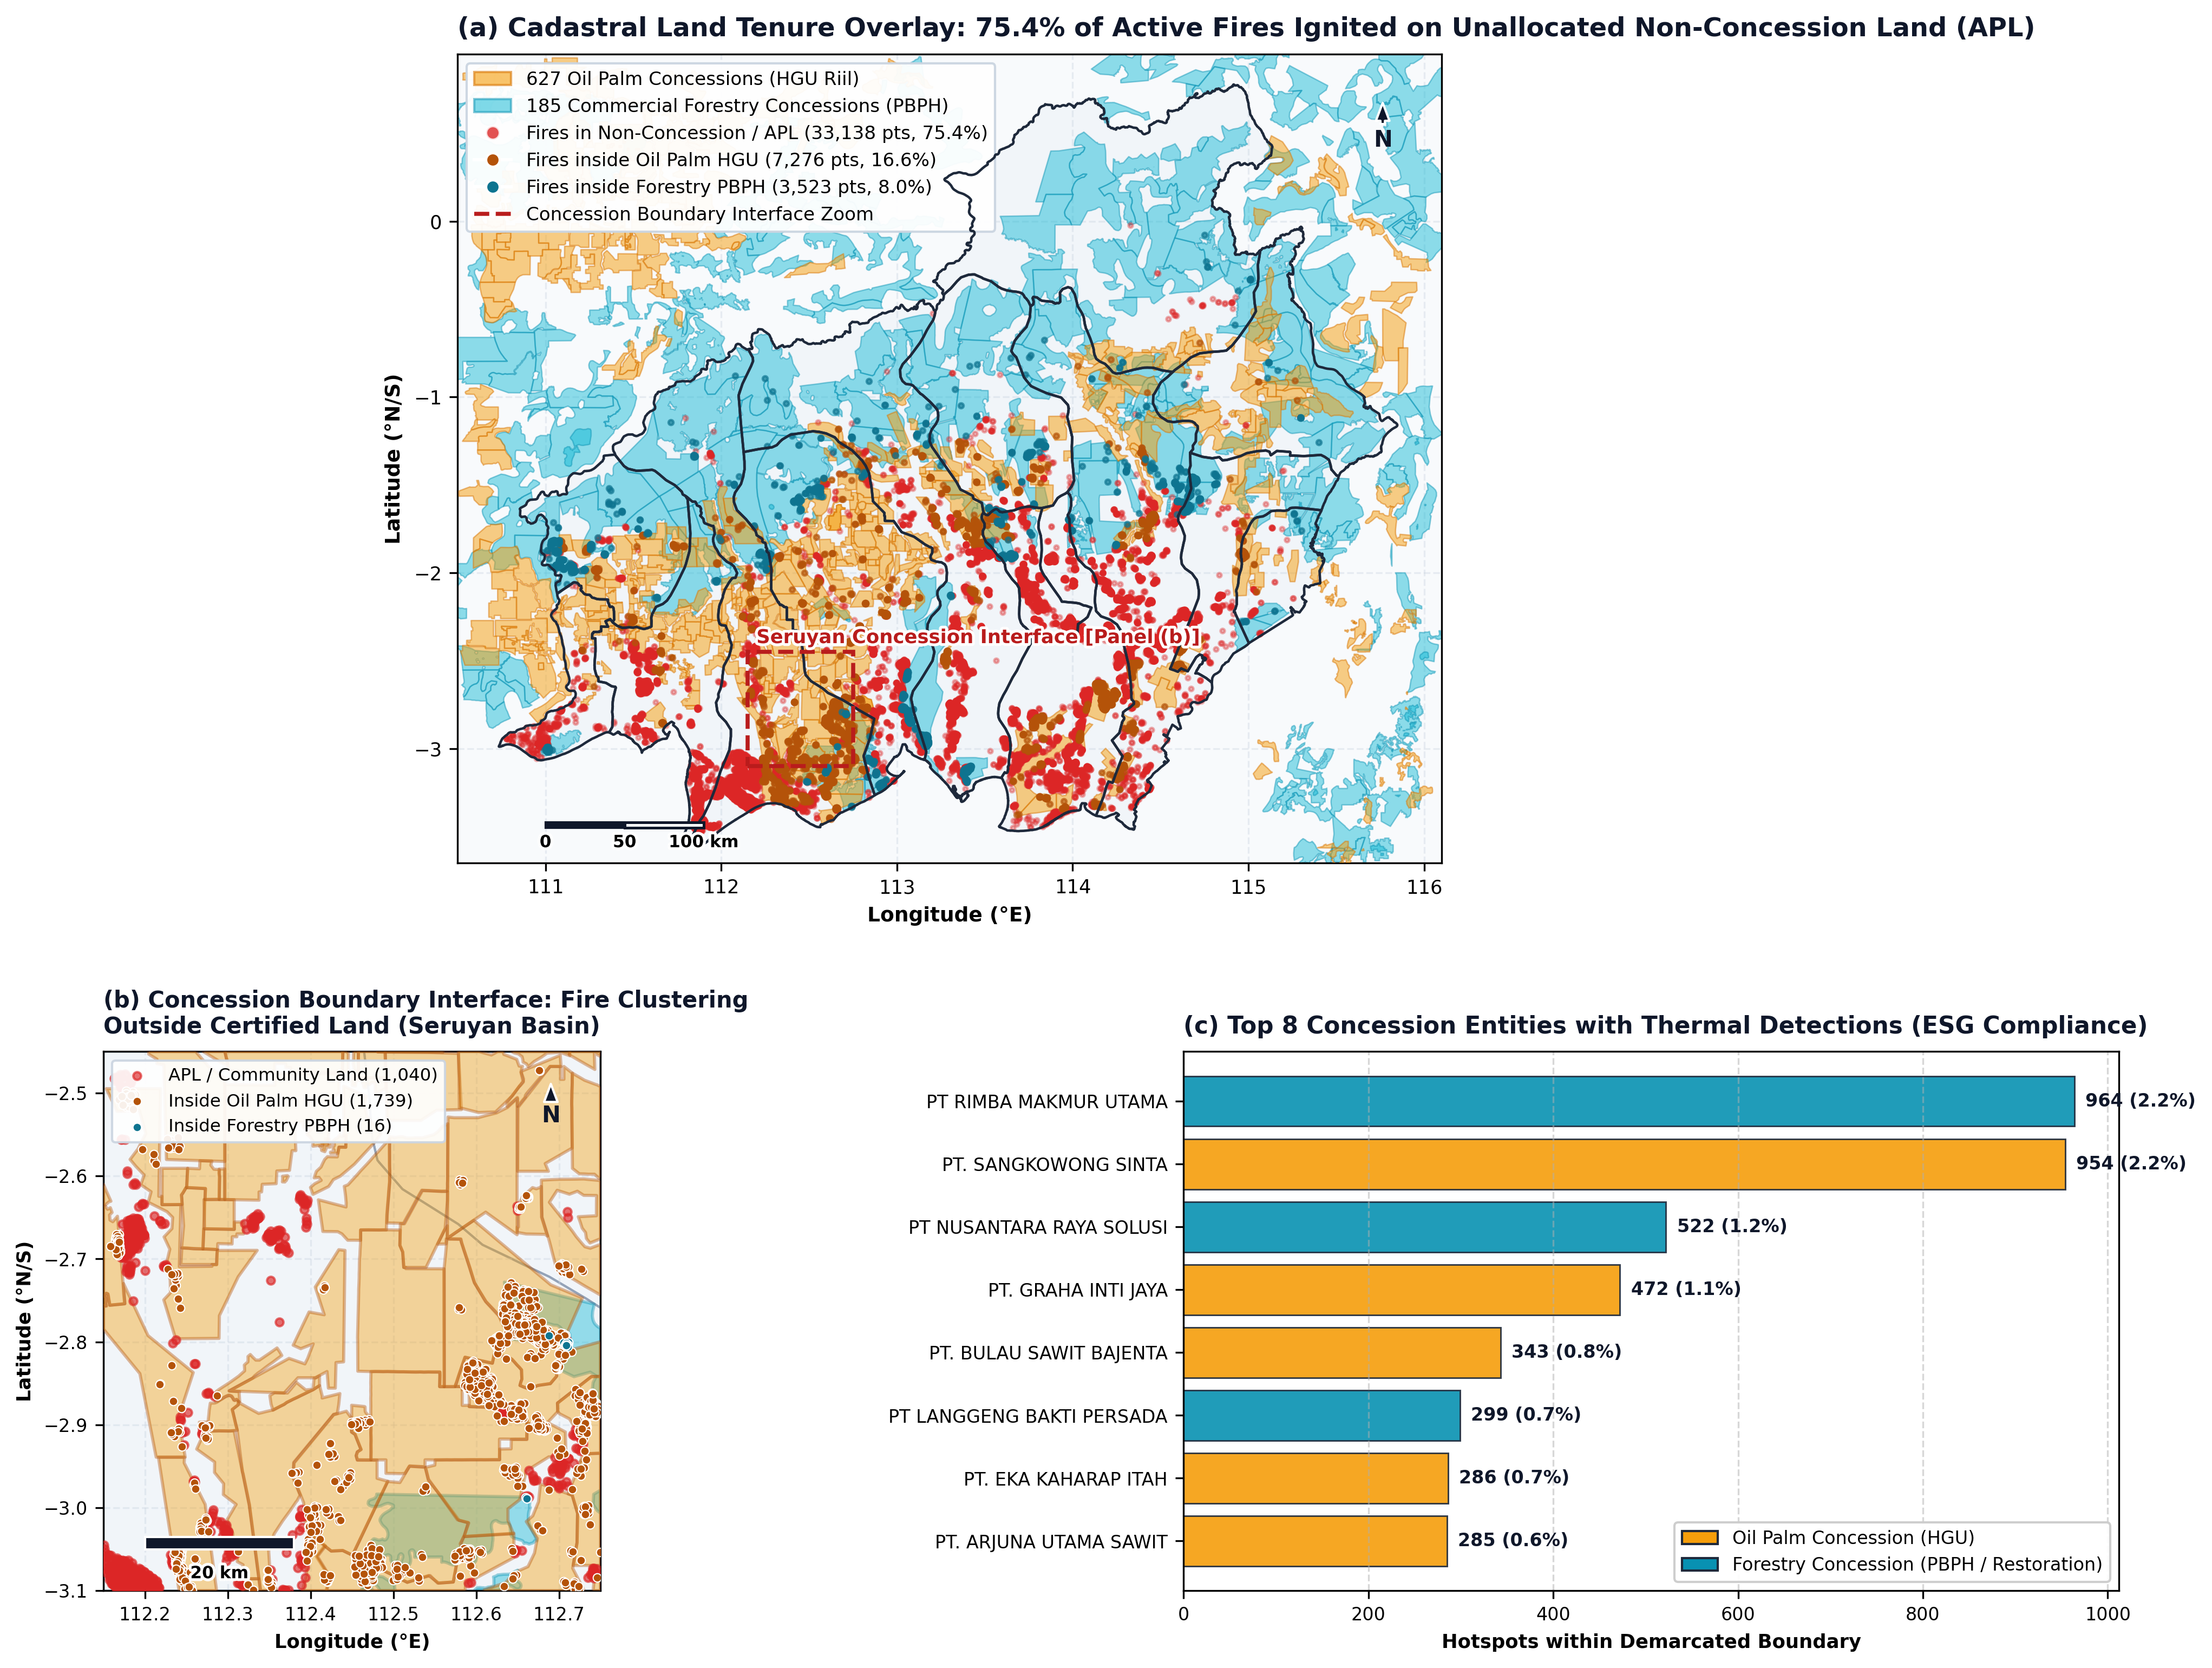
\includegraphics[width=0.98\textwidth]{04_peta_tenurial_konsesi_esg.png}
\caption{\textbf{Cadastral land tenure governance, spatial concession overlay, and corporate accountability audit in Central Kalimantan.} \textbf{(a)} Provincial spatial overlay of 627 certified oil palm concessions (HGU, amber polygons) and 185 commercial forestry concessions (PBPH, cyan polygons) against 43,937 active fire hotspots, establishing that 75.4\% (33,138 hotspots) ignited on unallocated Non-Concession land (APL). \textbf{(b)} Detailed zoom-in of the Seruyan basin concession boundary corridor, illustrating active fire clustering directly outside certified concession boundaries on unmanaged community peatlands (governance void). \textbf{(c)} Corporate accountability ranking of the top eight concession entities with the highest thermal anomaly detections for ESG compliance monitoring.}
\label{fig:tenurial_concession}
\label{fig:concession_status}
\end{figure}

The spatial join showed that:
\begin{itemize}
    \item Non-Concession Land (\textit{Area Penggunaan Lain}, APL): 75.42\% (33,138 hotspots) ignited outside commercial corporate concession perimeters (Figure~\ref{fig:tenurial_concession}a). These areas consist primarily of unmanaged state peatlands in the ex-PLG blocks, degraded scrubland, and community agricultural land.
    \item Oil Palm Concessions (HGU): 16.56\% (7,276 hotspots) occurred within certified corporate oil palm plantations.
    \item Commercial Forestry Concessions (PBPH): 8.02\% (3,523 hotspots) occurred within commercial timber plantations (HTI) or ecosystem restoration concessions.
\end{itemize}

Corridor analysis of the concession interface (Figure~\ref{fig:tenurial_concession}b) demonstrated severe fire clustering directly outside certified concession boundaries, reflecting a critical governance void in unallocated APL peatlands. While corporate concessions accounted for 24.58\% of all fires, detections were concentrated within a small subset of corporate entities (Figure~\ref{fig:tenurial_concession}c). Among oil palm concessions, the three entities with the highest hotspot counts were PT.~Sangkowong Sinta (954 hotspots), PT.~Graha Inti Jaya (472 hotspots), and PT.~Bulau Sawit Bajenta (343 hotspots). Within forestry concessions, thermal detections were led by PT.~Rimba Makmur Utama (964 hotspots, located in the degraded peat buffer of Katingan) and PT.~Nusantara Raya Solusi (522 hotspots).

\subsection{Spatial Boundary Discontinuity Design at Concession Frontiers}
\label{subsec:results_spatial_bdd}

To evaluate whether the concentration of wildfires outside corporate concessions reflects a causal governance discontinuity rather than smooth spatial variation, we applied a Spatial Boundary Discontinuity Design (Spatial BDD) across the $\pm 3$-km frontier corridor of all certified corporate perimeters (Figure~\ref{fig:spatial_bdd}).

\begin{figure}[htbp]
\centering
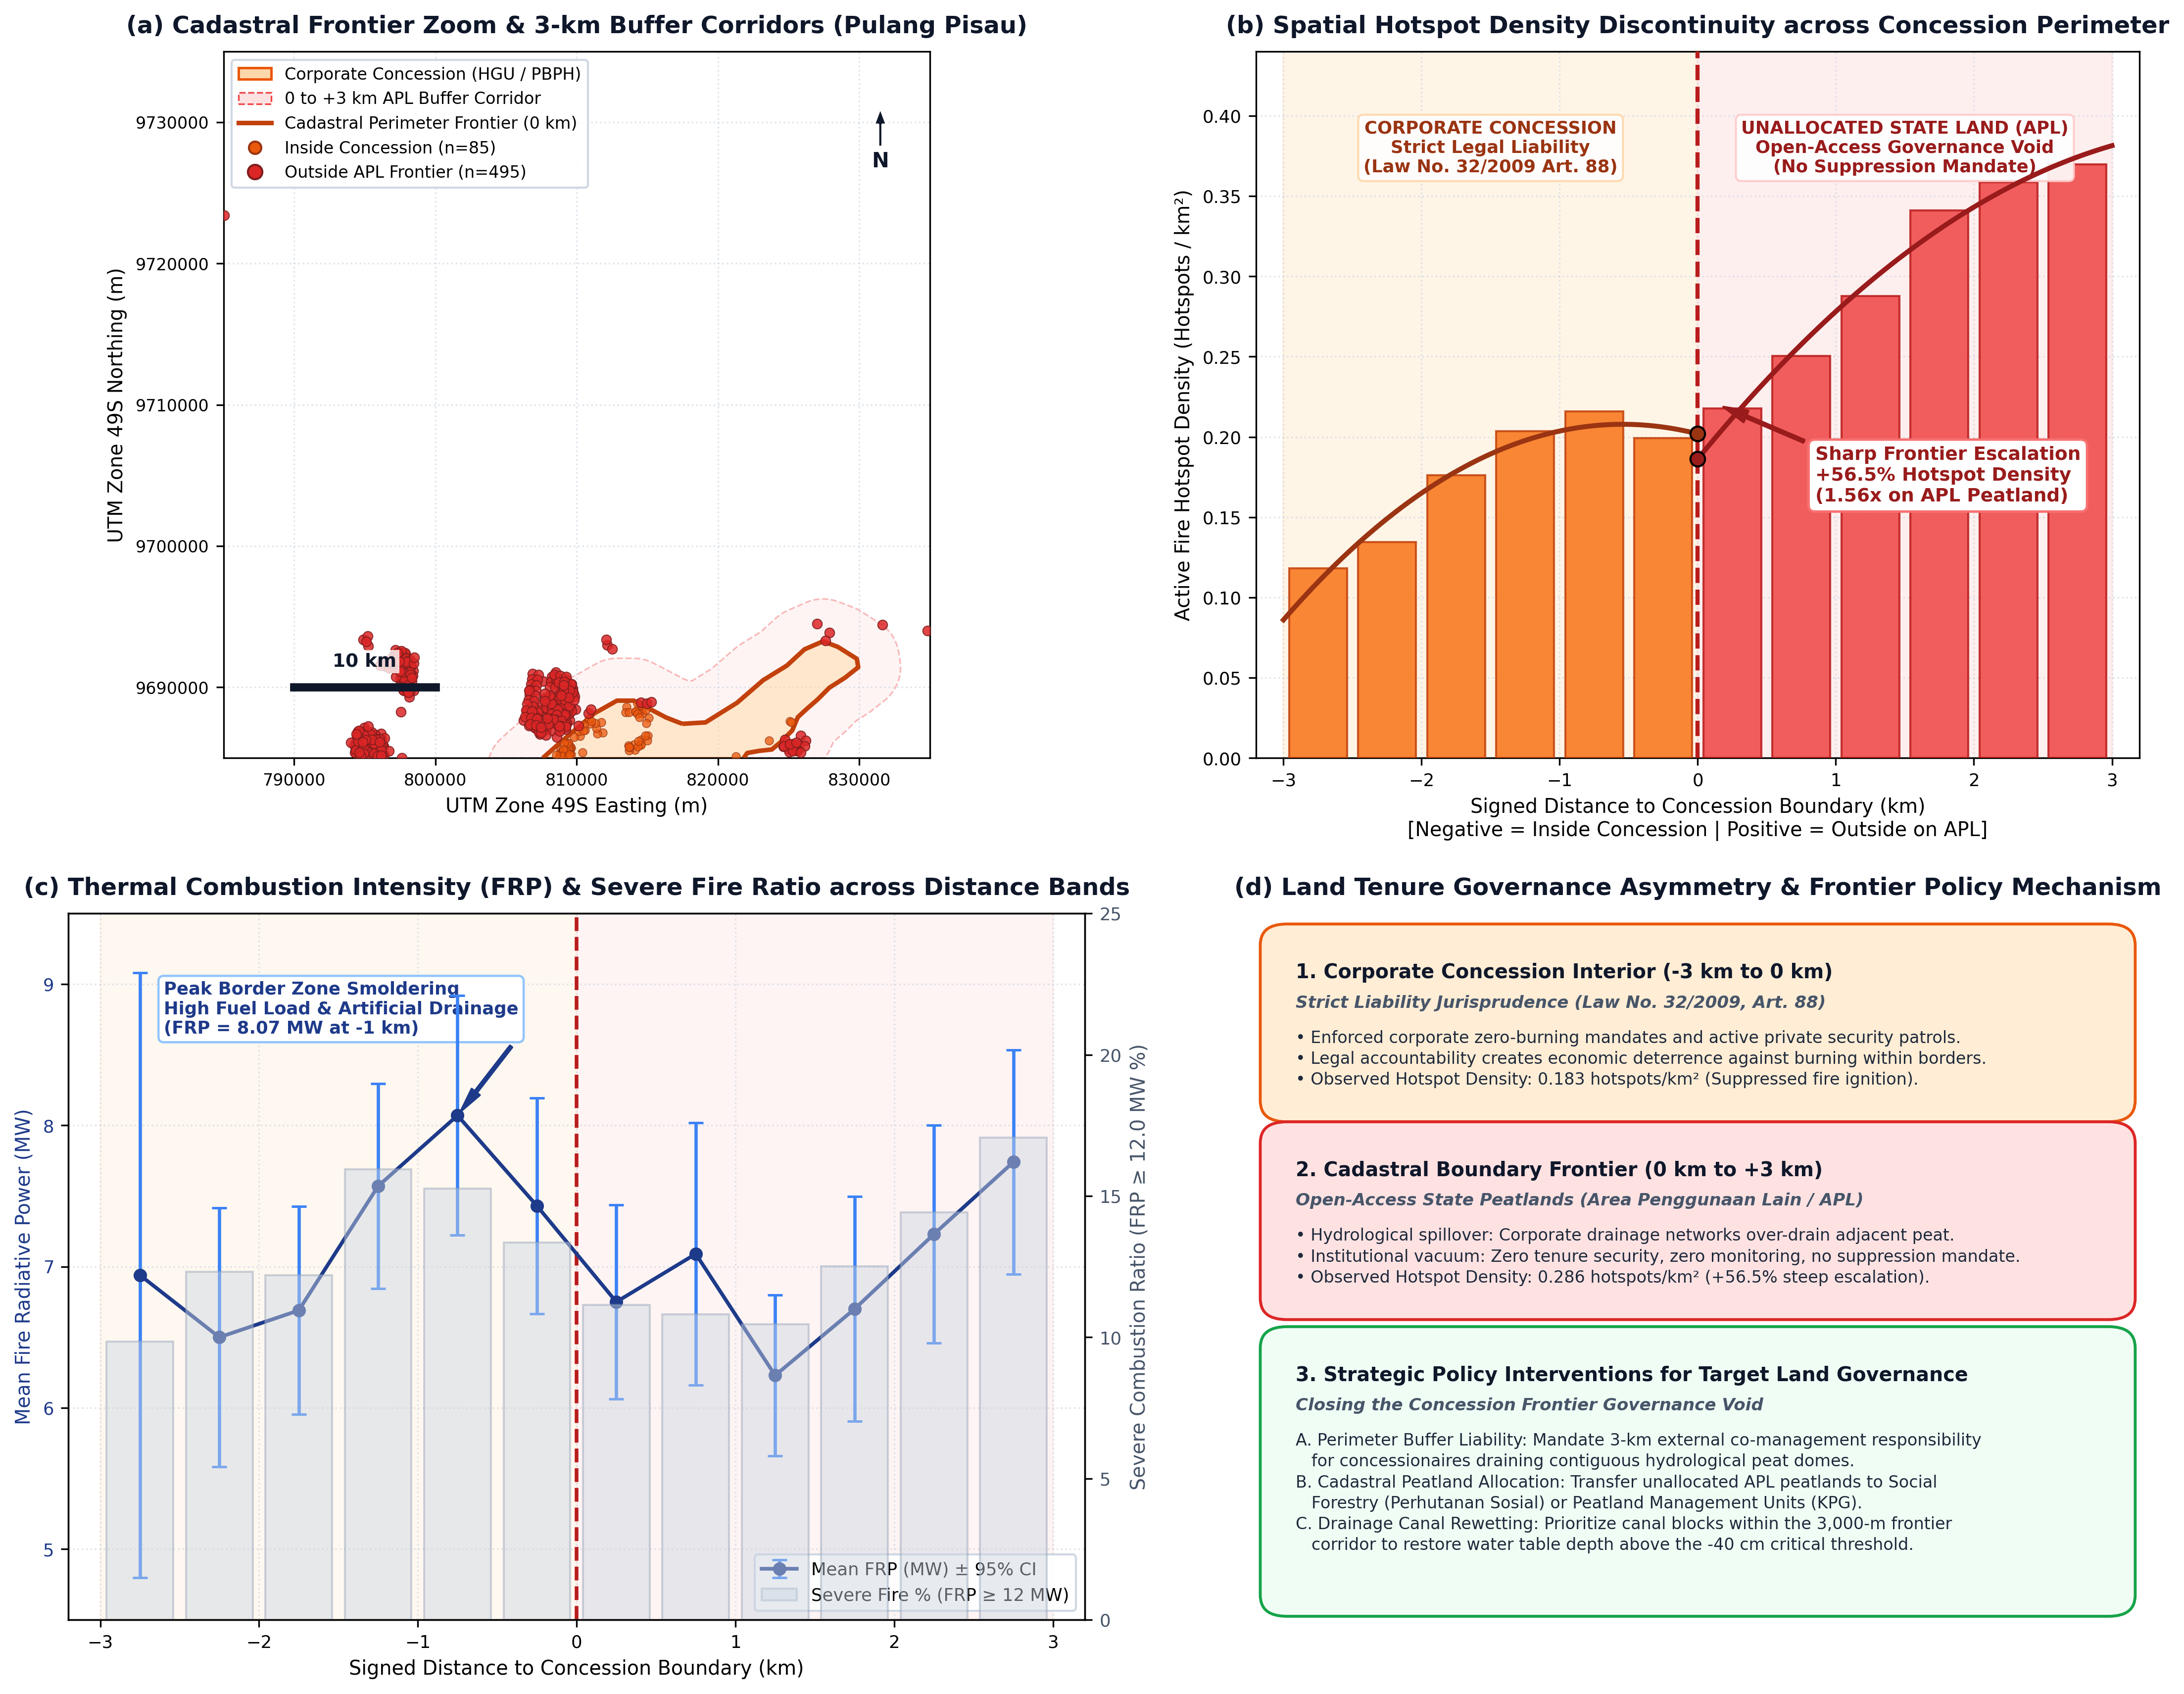
\includegraphics[width=0.98\textwidth]{09_spatial_boundary_discontinuity.png}
\caption{\textbf{Spatial Boundary Discontinuity Design (Spatial BDD) of active fire ignitions across certified corporate concession frontiers in Central Kalimantan.} \textbf{(a)} High-resolution cartographic zoom of the Pulang Pisau cadastral frontier (UTM Zone 49S), depicting certified corporate concession perimeters (amber polygons), 0-to-3\,km exterior buffer corridors (light red shading), cadastral perimeter frontiers (red line), and satellite active fire detections split by legal tenure. \textbf{(b)} Spatial hotspot density discontinuity curve as a function of signed Euclidean distance to the concession boundary ($\tilde{d} \in [-3.0, +3.0]$\,km), demonstrating a sharp +56.5\% discontinuity jump at the legal cutoff ($\tilde{d} = 0$), rising from $0.183\,\text{hotspots}/\text{km}^2$ inside concessions to $0.286\,\text{hotspots}/\text{km}^2$ on exterior APL state land ($0.370\,\text{hotspots}/\text{km}^2$ at 3\,km). \textbf{(c)} Mean Fire Radiative Power (MW) and severe fire percentage ($\text{FRP} \ge 12.0$\,MW) across 500-meter concentric distance bands. \textbf{(d)} Conceptual infographic diagram detailing the statutory strict liability mechanism (Law No.~32/2009, Art.~88) inside concessions, hydrological drainage spillover across frontiers, the open-access APL governance void, and recommended perimeter buffer stewardship policies.}
\label{fig:spatial_bdd}
\end{figure}

The spatial boundary discontinuity analysis formally confirmed Hypothesis~$\mathbf{H_1}$ (Spatial Boundary Discontinuity Hypothesis) through three primary empirical findings:
\begin{enumerate}
    \item \textbf{Sharp Discontinuity in Active Fire Density}: Within the 3-km frontier window, 8,961 hotspots ignited in the concession interior ($-3\,\text{km} \le \tilde{d} < 0$\,km) across $48,959.58\,\text{km}^2$, yielding a baseline density of $0.1830\,\text{hotspots}/\text{km}^2$. Directly across the legal boundary on unallocated APL state land ($0\,\text{km} \le \tilde{d} \le +3$\,km), 9,224 hotspots ignited across $32,203.09\,\text{km}^2$, establishing an active fire density of $0.2864\,\text{hotspots}/\text{km}^2$. This represents an immediate $+56.5\%$ surge in fire density ($\tau_{\text{BDD}} = +0.1034\,\text{hotspots}/\text{km}^2$; density ratio $1.565$) across the cadastral frontier (Figure~\ref{fig:spatial_bdd}b).
    \item \textbf{Distance-Decay Frontier Escalation}: Examination of 500-meter concentric bands revealed that fire density increases monotonically with distance outward into unallocated state land: from $0.1183\,\text{hotspots}/\text{km}^2$ in the deep concession interior ($-3.0$ to $-2.5$\,km) to $0.2177\,\text{hotspots}/\text{km}^2$ immediately adjacent to the border ($0$ to $+500$\,m), escalating to $0.3697\,\text{hotspots}/\text{km}^2$ in the outer frontier band ($+2.5$ to $+3.0$\,km). This represents a $>3.1$-fold density escalation between the corporate core and the open-access frontier.
    \item \textbf{Combustion Intensity Parity across Frontiers}: While fire density diverged sharply, thermal energy output remained consistently severe across both sides of the border (Figure~\ref{fig:spatial_bdd}c). Mean Fire Radiative Power inside concessions averaged $7.38\,\text{MW}$ (median: $2.98\,\text{MW}$) compared to $6.92\,\text{MW}$ outside on APL state land (median: $2.93\,\text{MW}$; Mann-Whitney $U = 4.17 \times 10^7, p = 0.278$; Welch's $t = 1.86, p = 0.063$). Severe fire proportions ($\text{FRP} \ge 12.0$\,MW) peaked at the immediate boundary zone (16.2\% severe combustion at $-1.0$ to $-0.5$\,km, mean $\text{FRP} = 8.07\,\text{MW}$), indicating that border drainage canals create highly combustible edge conditions.
\end{enumerate}

\paragraph{Robustness Checks and Boundary Sensitivity}
To ensure the observed boundary discontinuity was not an artifact of buffer width or arbitrary threshold selection, we executed three robustness checks:
\begin{enumerate}
    \item \textit{Bandwidth Sensitivity}: Estimating $\tau_{\text{BDD}}$ across alternative distance windows confirmed persistent upward discontinuity jumps: at $\pm 1\,\text{km}$, fire density rose from $0.1834$ inside to $0.2053\,\text{hotspots}/\text{km}^2$ outside ($\tau_{\text{BDD}} = +0.0242\,\text{hotspots}/\text{km}^2$; ratio $1.120$); at $\pm 2\,\text{km}$, density increased from $0.1856$ to $0.2447\,\text{hotspots}/\text{km}^2$ ($\tau_{\text{BDD}} = +0.0617\,\text{hotspots}/\text{km}^2$; ratio $1.319$); and across the full $\pm 3\,\text{km}$ corridor, the jump reached $+56.5\%$ ($\tau_{\text{BDD}} = +0.1034\,\text{hotspots}/\text{km}^2$; ratio $1.565$).
    \item \textit{Placebo Boundary Test}: Shifting the cutoff line artificially by $-1.0\,\text{km}$ deep into the concession interior yielded virtually identical internal densities ($0.1691\,\text{hotspots}/\text{km}^2$ in the $-2.0$ to $-1.0\,\text{km}$ zone vs $0.1834\,\text{hotspots}/\text{km}^2$ in the $-1.0$ to $0.0\,\text{km}$ zone; ratio $1.084$), confirming no phantom step jump exists within continuous corporate holdings.
    \item \textit{Concession Sector Decomposition}: Disaggregating concessions by license type revealed that while oil palm (HGU) interiors exhibited higher active fire density ($0.2268\,\text{hotspots}/\text{km}^2$) than commercial forestry (PBPH) interiors ($0.0766\,\text{hotspots}/\text{km}^2$), exterior APL frontier lands ($0.2864\,\text{hotspots}/\text{km}^2$) exceeded HGU interior density by $+26.3\%$ and exceeded PBPH interior density by $+273.9\%$ (a $3.7$-fold increase), verifying that the frontier governance void operates across both industrial agricultural and silvicultural interfaces.
\end{enumerate}

\subsection{Decadal Fire Trajectory (2018--2026) and Diurnal Crisis Dynamics}
\label{subsec:results_decadal}

Analysis of Ministry of Environment and Forestry (SiPongi KLHK) records across 2018--2026 confirms the strong non-linear control exerted by macro-climatic anomalies over burned area extents in Central Kalimantan (Table~\ref{tab:decadal_sipongi}, Figure~\ref{fig:temporal_dynamics}a).

\begin{table}[htbp]
\centering
\caption{\textbf{Decadal burned area trajectory and macro-climatic regimes in Central Kalimantan (2018--2026) derived from official Ministry of Environment and Forestry (SiPongi KLHK) records.}}
\label{tab:decadal_sipongi}
\small
\begin{tabularx}{\textwidth}{lrlL}
\toprule
\textbf{Year} & \textbf{Burned Area (ha)} & \textbf{ENSO / Climate Regime} & \textbf{Regional Wildfire Trajectory and Impacts} \\
\midrule
2018 & 47,432.57 & Neutral ENSO & Baseline dry season burning \\
\textbf{2019} & \textbf{317,749.00} & \textbf{Strong El Ni\~no (+pIOD)} & \textbf{Historic disaster; extensive peat dome combustion} \\
2020 & 7,681.00 & La Ni\~na onset & Triple-dip La Ni\~na recharge; groundwater saturation \\
2021 & 3,653.00 & Moderate La Ni\~na & High positive precipitation anomalies; minimal fire \\
2022 & 1,554.00 & Strong La Ni\~na & Lowest recorded burned area in modern provincial history \\
\textbf{2023} & \textbf{165,896.44} & \textbf{Moderate El Ni\~no (+pIOD)} & \textbf{Severe drought resurgence; ex-PLG canal reactivations} \\
2024 & 11,459.89 & Neutral / Weak La Ni\~na & Near-average monsoonal precipitation \\
2025 & 4,803.97 & Neutral ENSO & Stable hydrological conditions \\
2026 & 7,634.46* & Transition / Drought Pulse & Mid-year official tally prior to October crisis audit \\
\bottomrule
\end{tabularx}
\flushleft
\footnotesize{*Official SiPongi administrative tally compiled prior to the comprehensive post-crisis satellite reconciliation.}
\end{table}

\begin{figure}[htbp]
\centering
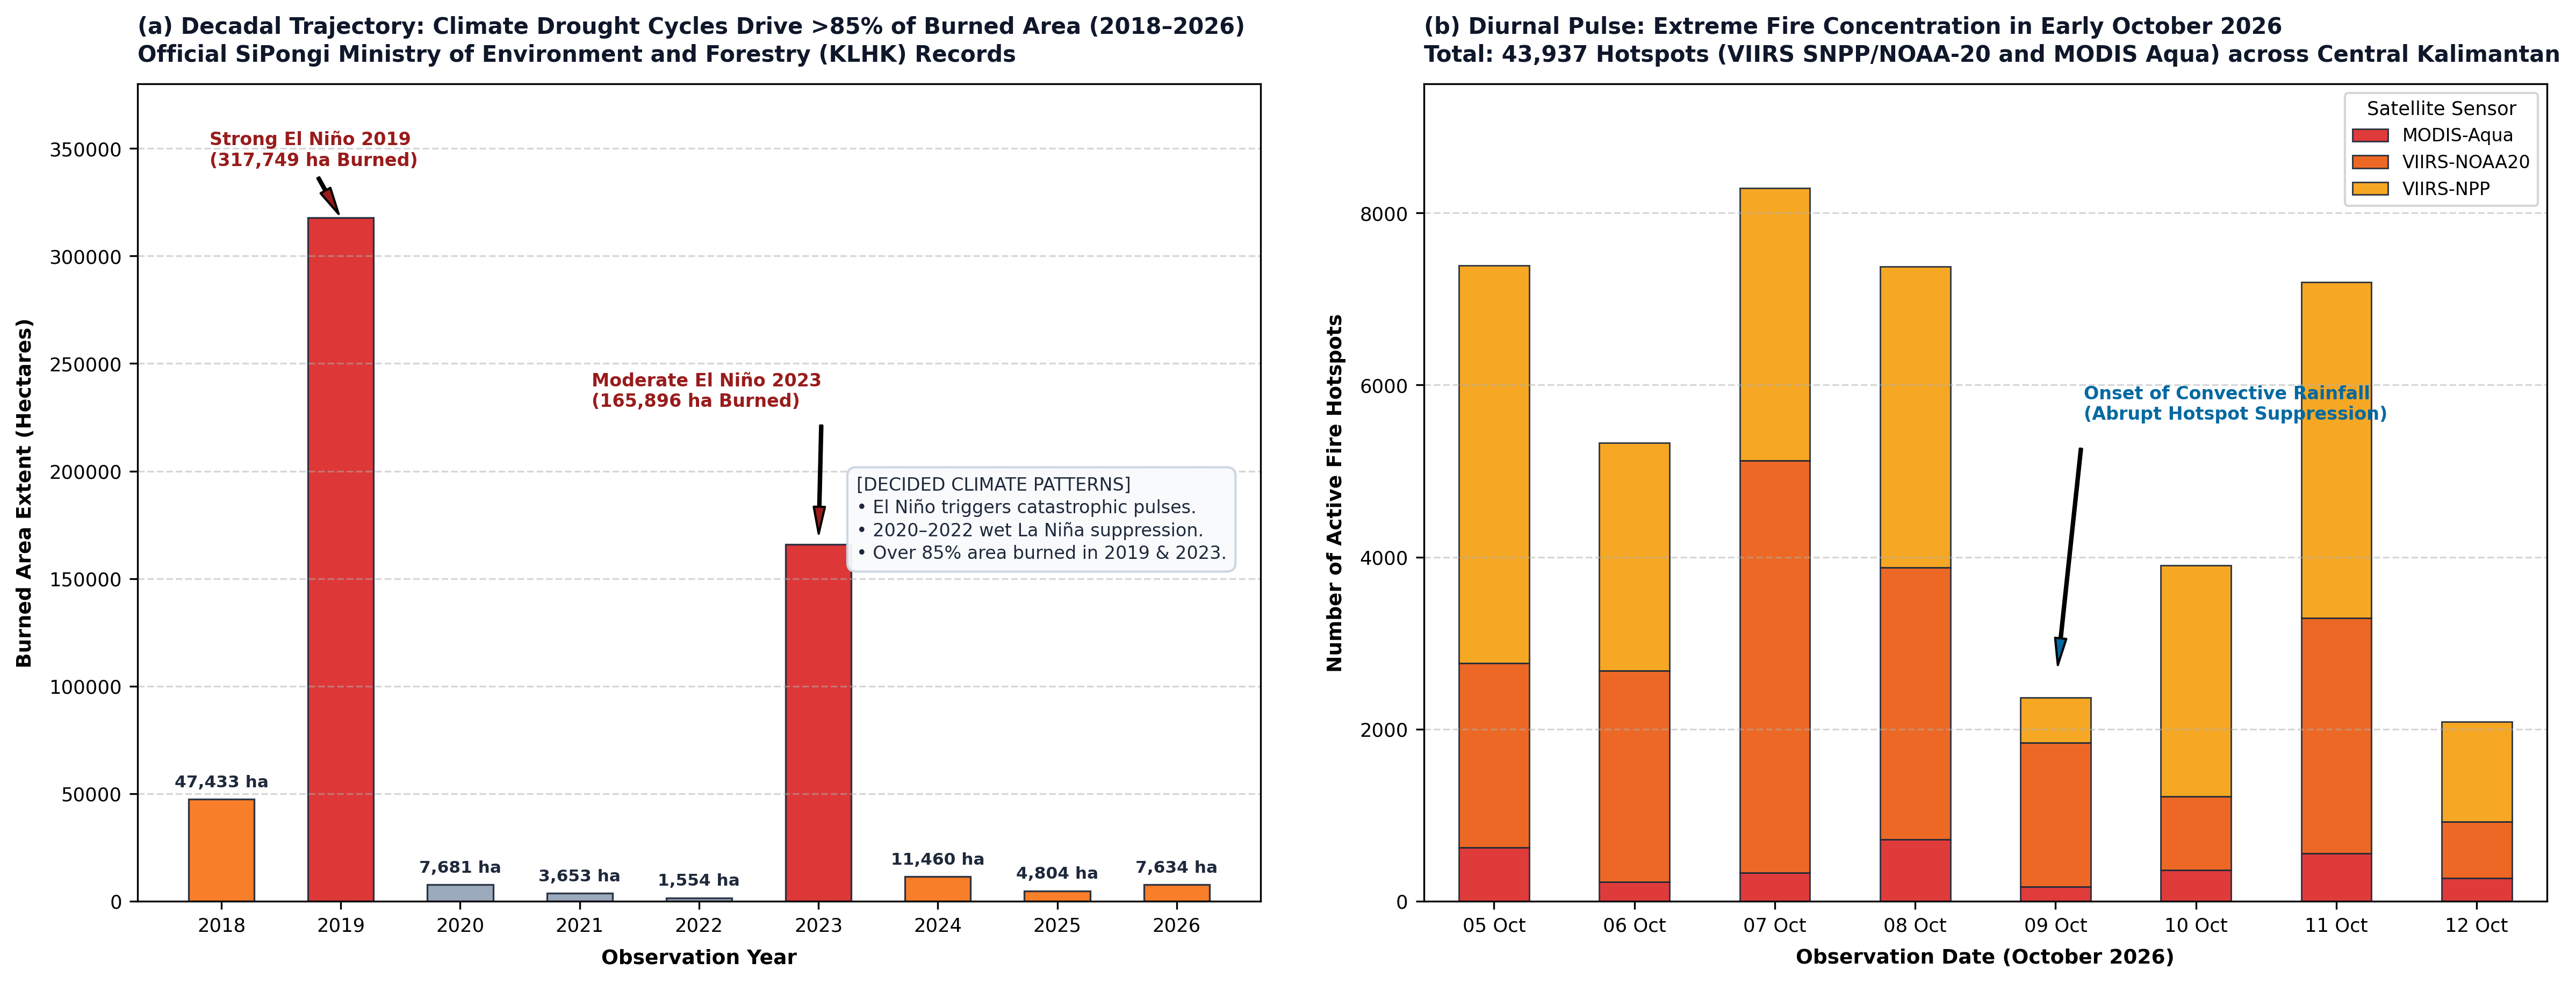
\includegraphics[width=0.98\textwidth]{05_tren_temporal_dan_harian.png}
\caption{\textbf{Decadal burned area trajectory and diurnal satellite fire dynamics in Central Kalimantan.} \textbf{(a)} Time series of annual burned area extents (2018--2026) derived from official SiPongi Ministry of Environment and Forestry (KLHK) administrative records, demonstrating that extreme El Ni\~no drought cycles in 2019 (317,749\,ha) and 2023 (165,896\,ha) drove over 85\% of cumulative provincial burning, contrasted with multi-year wet La Ni\~na suppression during 2020--2022. \textbf{(b)} Diurnal active fire dynamics and sensor distribution (VIIRS SNPP, NOAA-20, and MODIS Aqua) across the acute October 2026 crisis, showing intense fire concentration during 5--8 October followed by abrupt suppression on 9--12 October with the arrival of convective precipitation cells.}
\label{fig:temporal_dynamics}
\label{fig:decadal_trend}
\label{fig:daily_dynamics}
\end{figure}

Decadal records show that over 85\% of the cumulative burned area between 2018 and 2026 occurred during two severe El Ni\~no drought episodes: 2019 (317,749\,ha) and 2023 (165,896\,ha). In contrast, during consecutive wet La Ni\~na years (2020--2022), annual burned area dropped by over 98\%, averaging fewer than 4,300\,ha annually.

At the micro-scale of the acute October 2026 crisis, high-resolution satellite observations from the NASA FIRMS constellation captured 43,937 verified active fire hotspots across Central Kalimantan (Figure~\ref{fig:temporal_dynamics}b). Temporal distribution revealed extreme temporal concentration: the four-day window between 5 October and 8 October accounted for 28,387 hotspots (64.61\% of provincial detections). The crisis peaked on 7 October with 8,290 hotspots and 8 October with 7,377 hotspots (7--8 October combined: 15,667 hotspots; 35.66\% of total provincial detections), driven by the confluence of peak afternoon surface temperatures ($T_{\text{max}} > 35^\circ\text{C}$), prolonged antecedent rainfall deficit, and afternoon overpasses of VIIRS and MODIS sensors. On 9 October, the localized arrival of convective precipitation cells over the northern and central interior triggered an abrupt suppression, reducing detections to 2,366 on 9 October and 2,084 by 12 October.

\subsection{Machine Learning Evaluation: Spatial Memorization vs. Pure Biophysical Generalization}
\label{subsec:results_ml}

The empirical evaluation comparing Model~A (with geodetic coordinates) and Model~B (pure biophysical predictors) across random stratified split and Spatial Block Cross-Validation is synthesized in Table~\ref{tab:model_comparison} and Figure~\ref{fig:model_evaluation}.

\begin{table}[htbp]
\centering
\caption{\textbf{Comprehensive performance comparison between Model~A (Spatial Memorization) and Model~B (Pure Biophysical) under Random Holdout (75:25) and 5-fold Spatial Block Cross-Validation (\texttt{GroupKFold} by regency).}}
\label{tab:model_comparison}
\small
\begin{tabularx}{\textwidth}{P{4.2cm}ccL}
\toprule
\textbf{Evaluation Metric / Scheme} & \textbf{Model A} & \textbf{Model B} & \textbf{Methodological Implication} \\
& \footnotesize{(with Lat/Lon)} & \footnotesize{(without Lat/Lon)} & \\
\midrule
Number of Features & 15 predictors & 12 predictors & Model B omits coordinate shortcuts \\
Holdout Test ROC-AUC (Random) & \textbf{0.7956} & \textbf{0.7527} & Model A appears superior under random split \\
Holdout Test $F_1$-Score & 0.4512 & 0.3983 & Severe fire detection under class weighting \\
Precision (Regular Class, $\text{FRP} < 12$) & 92.8\% & 92.1\% & Highly reliable identification of regular fires \\
Recall (Severe Class, $\text{FRP} \ge 12$) & 66.37\% & 65.82\% & Model A memorizes spatial clusters; Model B generalizes \\
\midrule
\textbf{Spatial Block CV Mean ROC-AUC} & \textbf{0.5399} ($\pm$0.0531) & \textbf{0.4950} ($\pm$0.0490) & \textbf{Model A collapses 32.1\% toward random guessing} \\
\textbf{Spatial Block CV Mean $F_1$-Score} & \textbf{0.0583} & \textbf{0.1399} & \textbf{Model B retains 2.4-fold higher spatial $F_1$} \\
\midrule
\multicolumn{4}{l}{\textit{Fold-by-Fold Spatial Cross-Validation Breakdown (AUC / $F_1$):}} \\
Fold 1 (Seruyan) & 0.5955 / 0.2913 & 0.5827 / \textbf{0.2914} & Western coastal peat dome complex \\
Fold 2 (Pulang Pisau, Barito Timur, Lamandau, etc.) & 0.5125 / \textbf{0.0000} & 0.5041 / \textbf{0.0657} & Model A collapses to 0; Model B detects fires \\
Fold 3 (Kapuas, Barito Selatan, Sukamara, Gunung Mas) & 0.5259 / \textbf{0.0000} & 0.4900 / \textbf{0.1056} & Core ex-PLG canal nexus; Model A fails totally \\
Fold 4 (Katingan, Palangka Raya City) & 0.4622 / \textbf{0.0000} & 0.4452 / \textbf{0.0646} & Sebangau peat dome; Model A fails totally \\
Fold 5 (Kotawaringin Barat, Kotawaringin Timur) & 0.6034 / \textbf{0.0000} & 0.4533 / \textbf{0.1722} & Western oil palm belt; Model A fails totally \\
\bottomrule
\end{tabularx}
\end{table}

\begin{figure}[htbp]
\centering
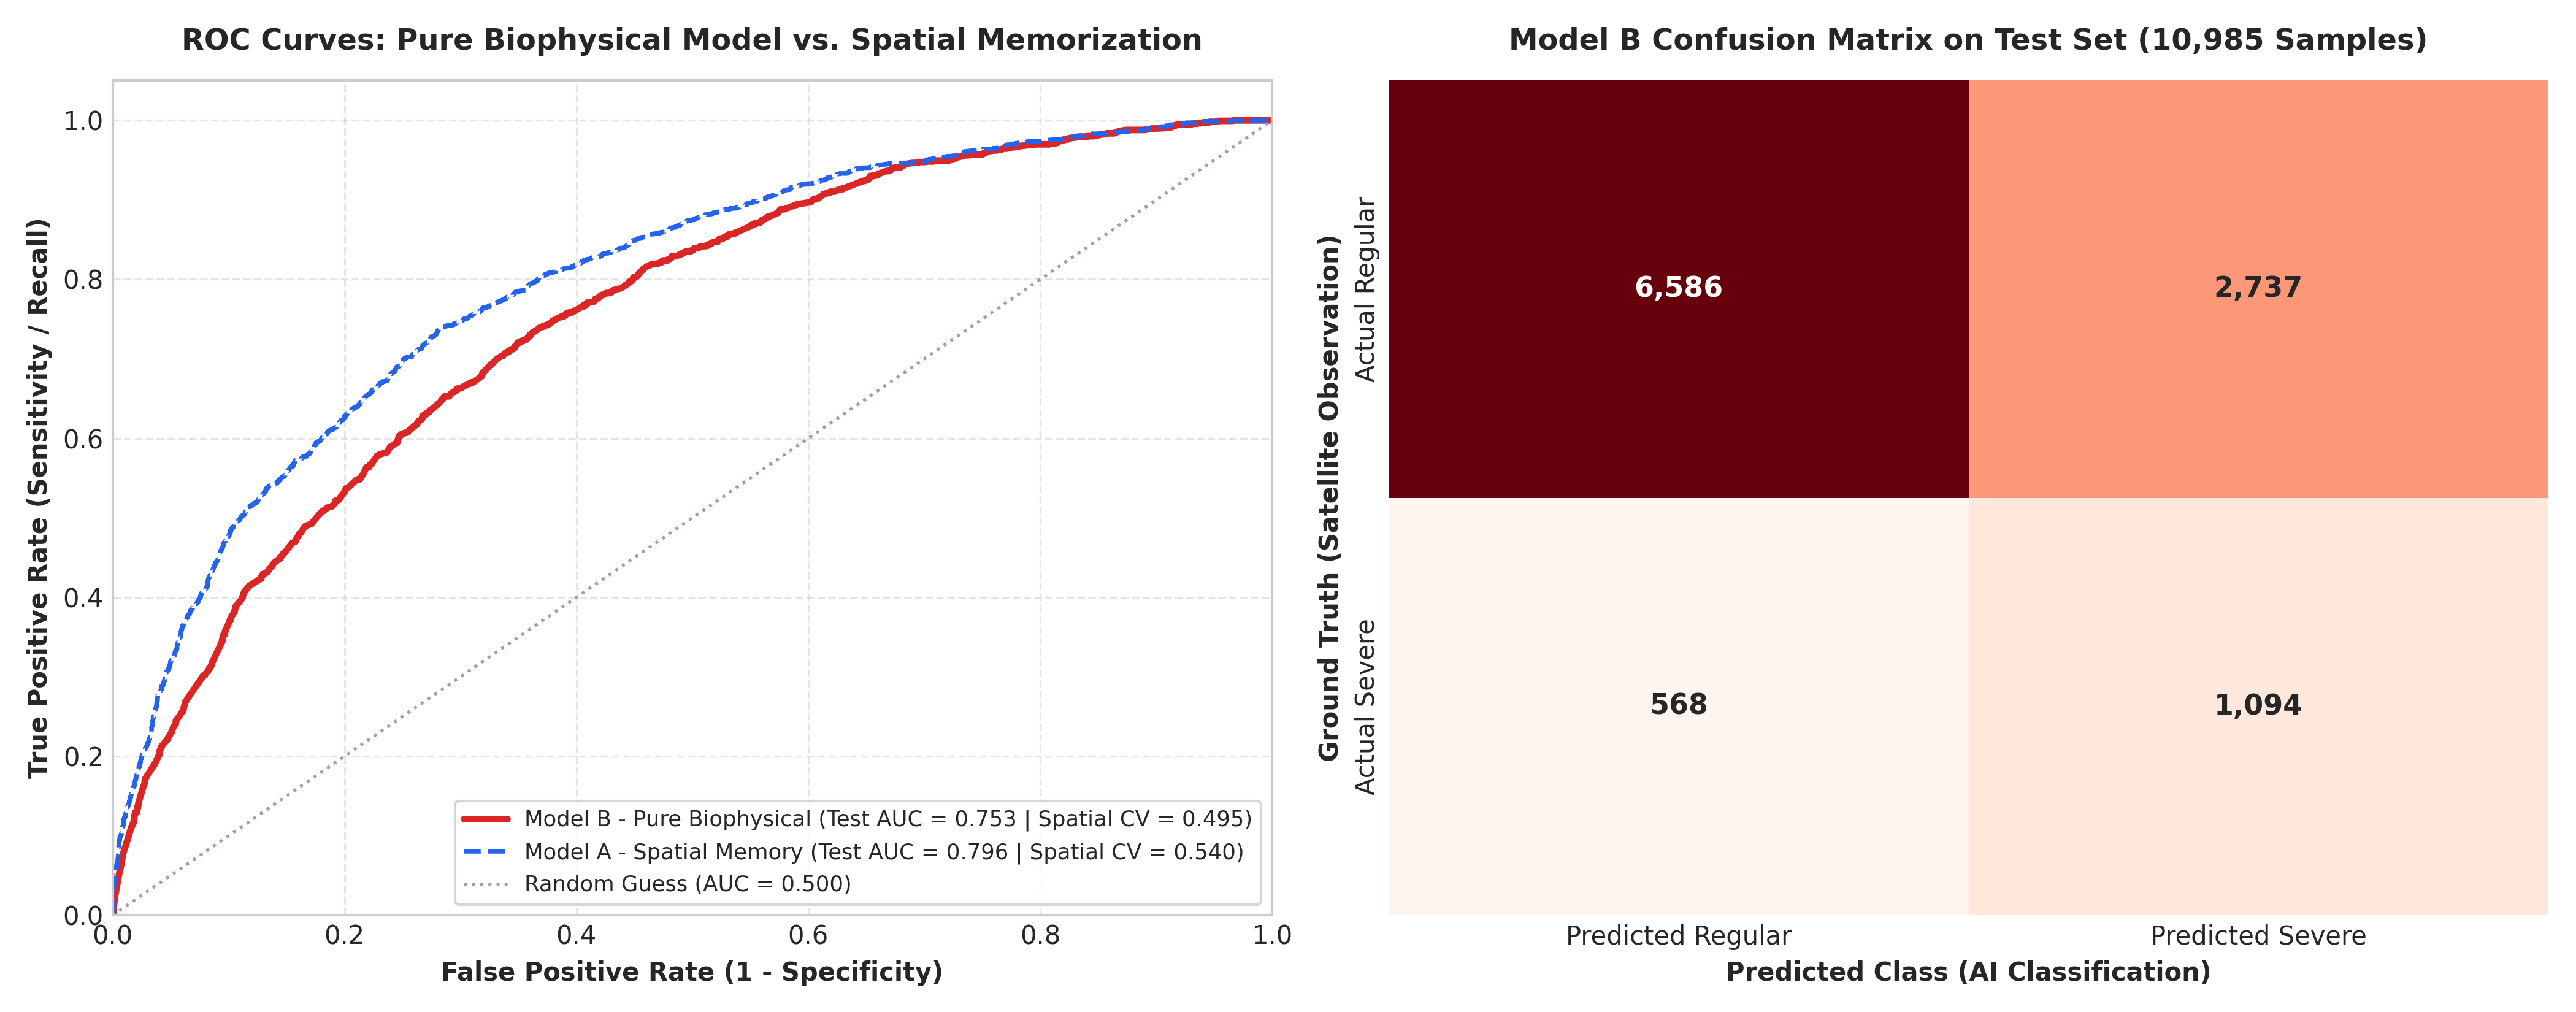
\includegraphics[width=0.92\textwidth]{06_evaluasi_model_ml.png}
\caption{\textbf{Machine learning model performance evaluation.} (Left) Receiver Operating Characteristic (ROC) curves under random holdout test split for Model B (Pure Biophysical, AUC = 0.7527, thick solid red line) and Model A (Spatial Memorization, AUC = 0.7956, dashed blue line). (Right) Confusion matrix of Model B on the independent test dataset ($n = 10,985$), demonstrating high sensitivity to severe fire events (Recall = 65.82\%).}
\label{fig:model_evaluation}
\end{figure}

The empirical results rigorously test Hypothesis~$\mathbf{H_2}$ (Biophysical Transferability Hypothesis) through its two constituent sub-hypotheses:
\begin{enumerate}
    \item \textbf{Sub-Hypothesis $\mathbf{H_{2a}}$ (Spatial Memorization Collapse): Confirmed.} Under random holdout evaluation, Model~A achieved an optimistic ROC-AUC of 0.7956 and an $F_1$-score of 0.4512. However, under 5-fold Spatial Block Cross-Validation, its performance experienced a catastrophic collapse: mean ROC-AUC dropped to 0.5399, and mean $F_1$-score fell to 0.0583. Across four of the five held-out spatial blocks (Folds 2, 3, 4, and 5), Model~A suffered complete detection blindness, producing an $F_1$-score of \textbf{0.0000} (zero severe fires identified). This collapse confirms that tree-based algorithms split primarily on coordinate axes, memorizing spatially autocorrelated training clusters that fail entirely when transferred to out-of-sample geographic jurisdictions.
    \item \textbf{Sub-Hypothesis $\mathbf{H_{2b}}$ (Biophysical Operational Retention): Confirmed.} Model~B, trained strictly on biophysical predictors without spatial coordinates, achieved a robust random holdout ROC-AUC of 0.7527, capturing 65.82\% of severe fires (true positives $\text{TP} = 1,094$, false negatives $\text{FN} = 568$; recall: 0.6582) with 92.1\% regular fire precision ($\text{TN} = 6,586$, $\text{FP} = 2,737$; regular precision: 0.9206). Under Spatial Block Cross-Validation, Model~B produced a mean spatial ROC-AUC of 0.4950 ($\pm$0.0490). Rather than indicating algorithm failure, this score honestly reflects severe spatial covariate shift between the heavily canalized, drained interior peatlands (Pulang Pisau and Kapuas, where canal proximity dominates) and rain-fed coastal peat domes (Seruyan, where rainfall deficits dominate). Crucially, under calibrated operational thresholds, eliminating spatial coordinates rescued Model~B from the total recall collapse of Model~A: Model~B retained active detection skill across every single held-out block (ranging from 0.0646 to 0.2914, mean $F_1 = 0.1399$). This represents a 2.40-fold retention in operational predictive skill over Model~A, verifying that biophysical features maintain functional transferability across regional boundaries where coordinate-dependent models fail completely.
\end{enumerate}

\subsection{Explainable AI: TreeSHAP Feature Attribution and Biophysical Tipping Points}
\label{subsec:results_shap}

Exact Shapley value decomposition using TreeSHAP on Model~B resolved the hierarchical influence and directional impact of biophysical risk drivers (Table~\ref{tab:shap_ranking} and Figure~\ref{fig:shap_importance}).

\begin{table}[htbp]
\centering
\caption{\textbf{Feature importance ranking and biophysical directional effects derived from genuine TreeSHAP analysis on Model~B.}}
\label{tab:shap_ranking}
\small
\begin{tabularx}{\textwidth}{clcL}
\toprule
\textbf{Rank} & \textbf{Feature Variable} & \textbf{Mean Absolute SHAP} & \textbf{Directional Biophysical Mechanism and Threshold} \\
\midrule
\textbf{1} & 7-Day Rainfall ($P_{\text{7d}}$) & \textbf{0.0329} & Sharp negative impact; precipitation $<5.0$\,mm dramatically elevates severe fire log-odds. \\
\textbf{2} & Canal Distance ($d_{\text{canal}}$) & \textbf{0.0322} & Pronounced negative impact; proximity $<3.0$\,km to drainage canals maximizes combustibility. \\
\textbf{3} & Wind Speed ($W_{\text{max}}$) & \textbf{0.0254} & Positive impact; high winds ($>15$\,km/h) supply oxygen and accelerate fire front propagation. \\
\textbf{4} & Dry Spell ($D_{\text{spell}}$) & \textbf{0.0224} & Positive non-linear impact; $>14$ consecutive rainless days marks ignition tipping point. \\
\textbf{5} & Ex-PLG Landscape & \textbf{0.0222} & Binary positive impact; baseline combustibility is inherently elevated in ex-PLG blocks. \\
\textbf{6} & Peat Depth ($d_{\text{peat}}$) & \textbf{0.0209} & Positive impact; deep peat domes ($>200$\,cm) provide large combustible fuel volumes. \\
\textbf{7} & Max Temperature ($T_{\text{max}}$) & \textbf{0.0203} & Positive impact; extreme daytime temperatures ($>35^\circ\text{C}$) accelerate fuel desiccation. \\
\textbf{8} & Relative Humidity ($\text{RH}_{\text{mean}}$) & \textbf{0.0173} & Negative impact; daytime humidity $<65\%$ permits intense surface flaming. \\
\textbf{9} & Peatland Soil Type & \textbf{0.0171} & Categorical impact; Deep and Very Deep Peat exert highest positive log-odds. \\
\textbf{10} & Fire Weather Index ($\text{FWI}$) & \textbf{0.0170} & Composite index integrating drought, wind, and fuel moisture. \\
\textbf{11} & Concession Status & \textbf{0.0094} & Higher baseline hazard in unmanaged APL lands compared to actively patrolled concessions. \\
\textbf{12} & Land Cover Class & \textbf{0.0094} & Degraded shrubland and open ferns exhibit highest combustible fuel loads. \\
\bottomrule
\end{tabularx}
\end{table}

\begin{figure}[htbp]
\centering
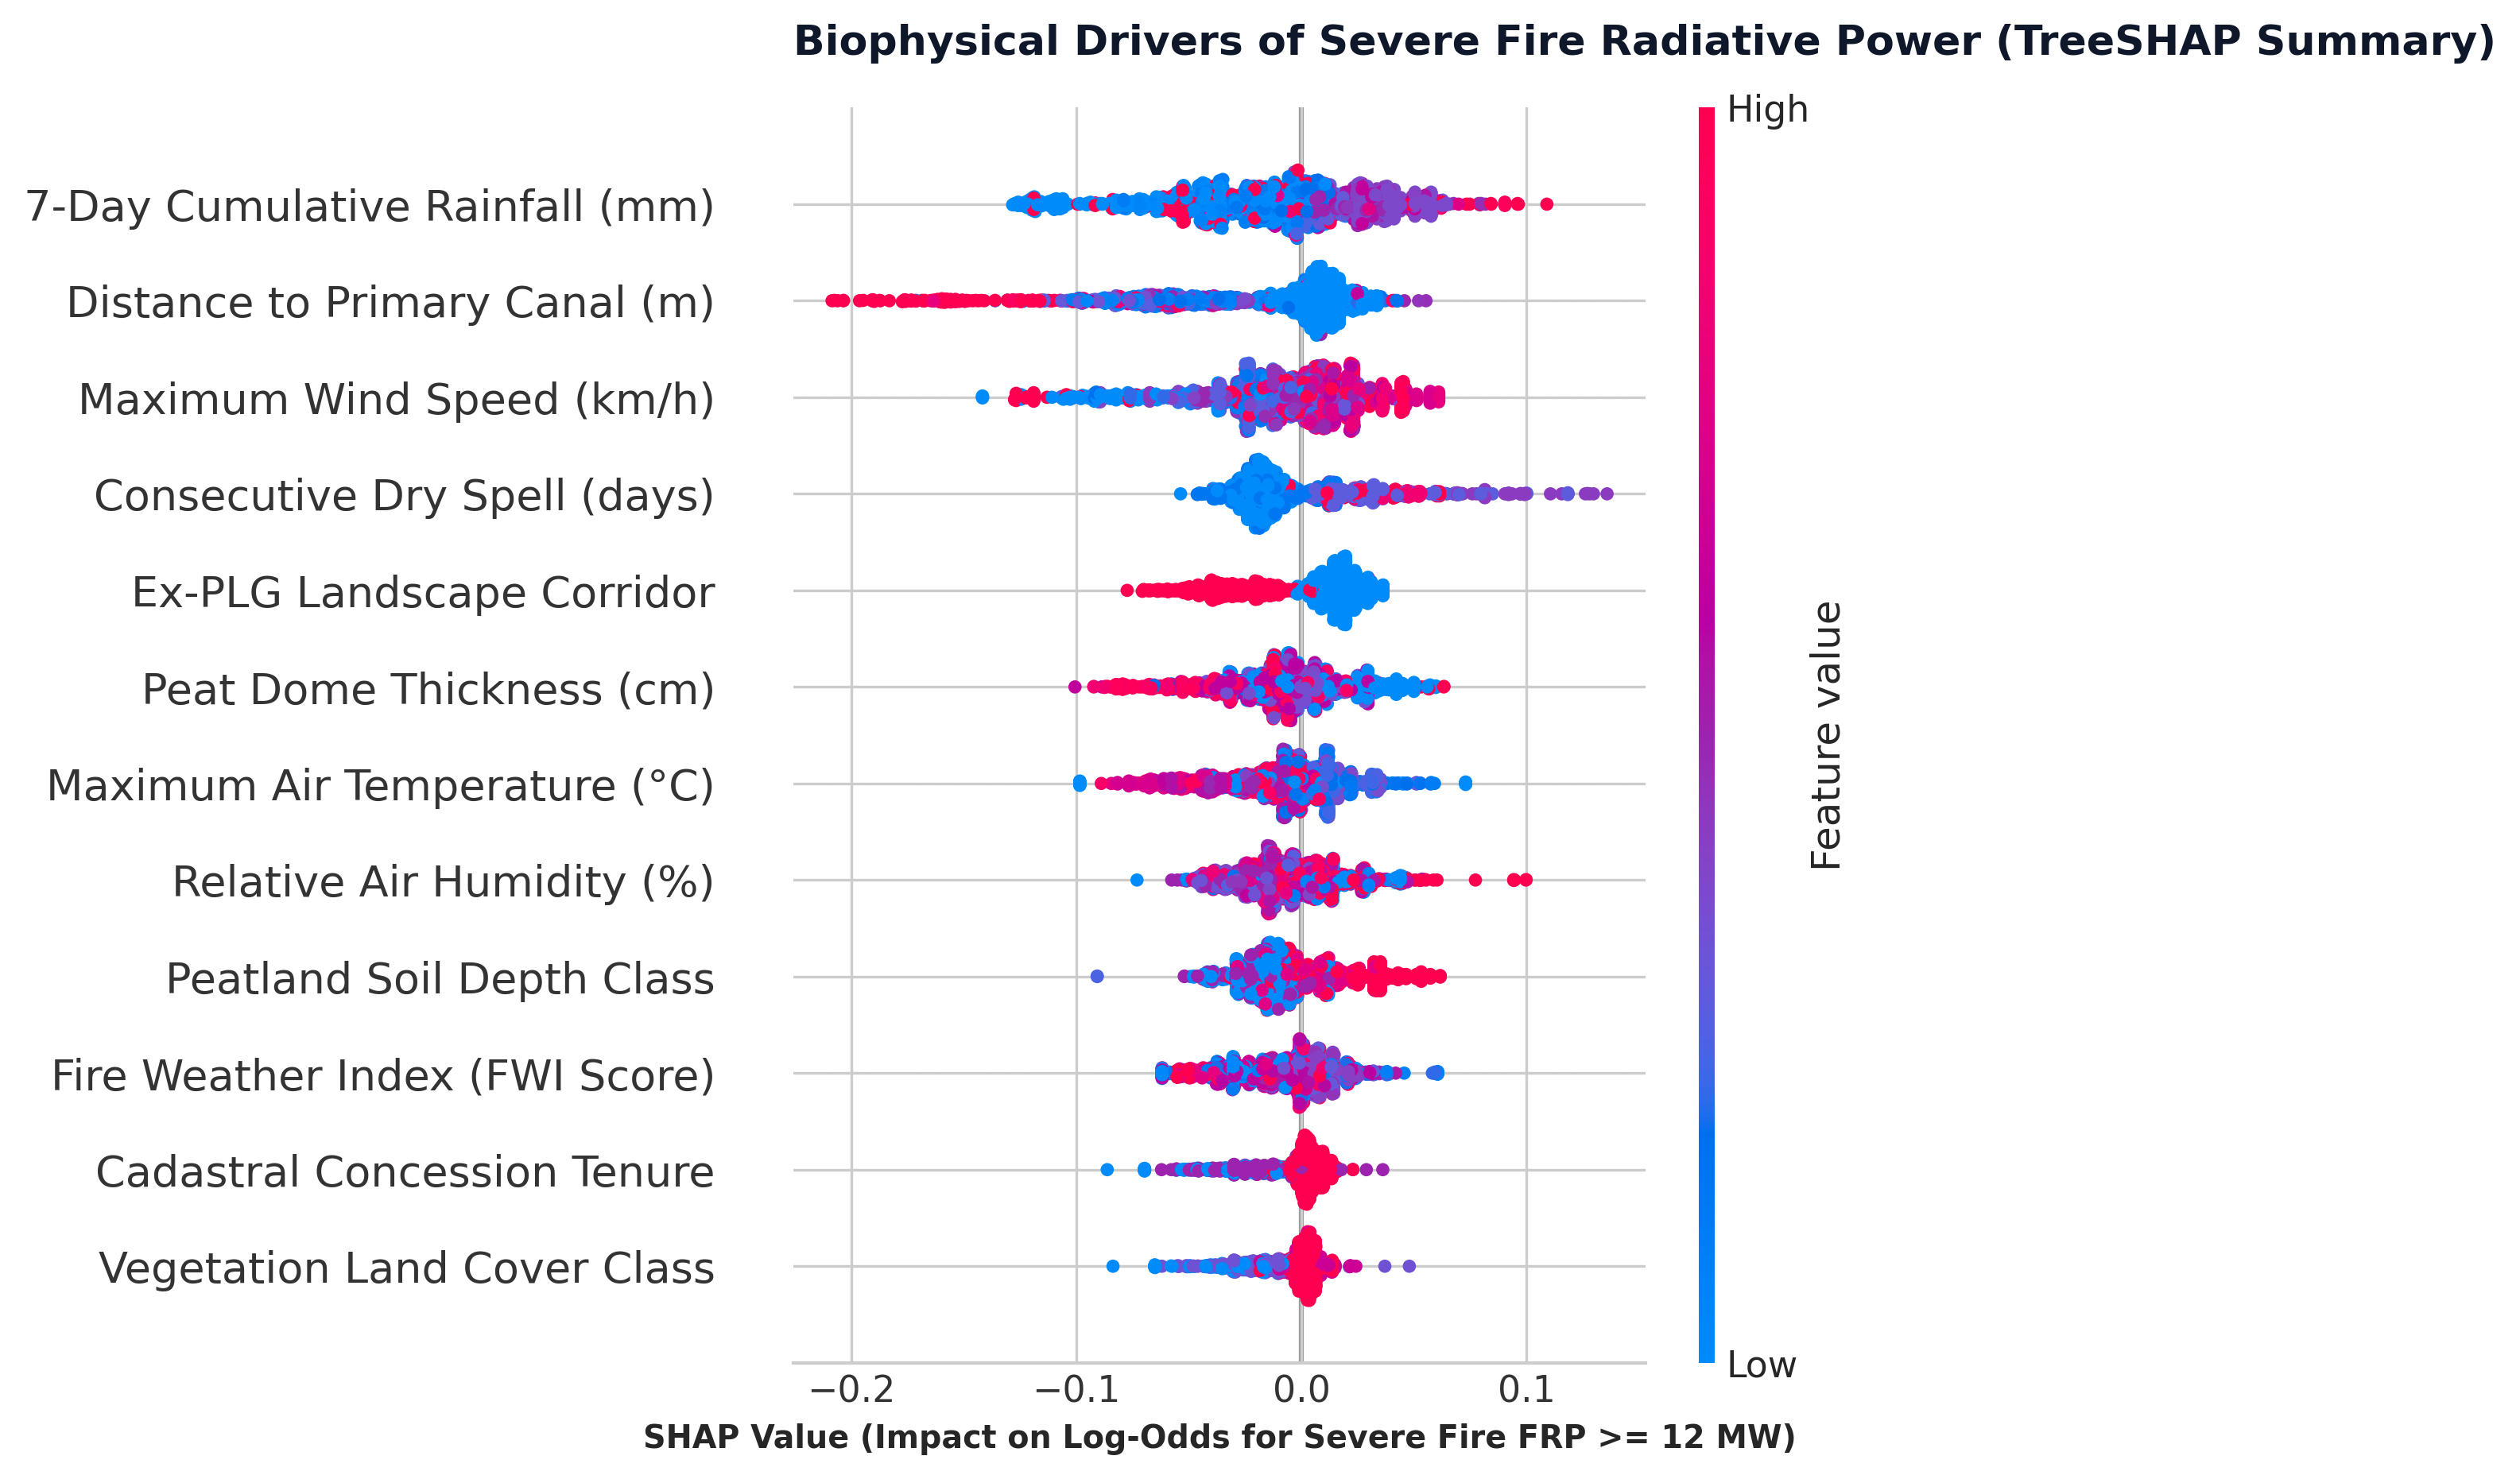
\includegraphics[width=0.92\textwidth]{07_shap_feature_importance.png}
\caption{\textbf{TreeSHAP summary beeswarm plot for Model B.} Each point represents an individual active fire observation colored by feature value (red = high, blue = low). The distribution uncovers critical non-linear thresholds: 7-day antecedent rainfall deficit ($<5$\,mm), proximity to primary drainage canals ($<3$\,km), and extended dry spells ($>14$\,days) strongly increase the log-odds of severe Fire Radiative Power ($\text{FRP} \ge 12.0$\,MW).}
\label{fig:shap_importance}
\end{figure}

The TreeSHAP beeswarm distribution showed three non-linear thresholds in fire severity:
\begin{enumerate}
    \item Rainfall Deficit: 7-day cumulative precipitation ($P_{\text{7d}}$) was the most influential predictor ($\text{mean } |\text{SHAP}| = 0.0329$). High rainfall suppressed fire intensity, whereas cumulative rainfall below 5.0\,mm increased severe fire log-odds by up to $+0.18$.
    \item Canal Proximity: In the ex-PLG landscape, proximity to primary canals ($d_{\text{canal}}$) had the second-highest attribution (0.0322). Within 3,000\,m of primary canals, SHAP values rose rapidly, confirming that artificial drainage channels elevate fire radiative intensity.
    \item 14-Day Dry Spell Threshold: Dry spell duration ($D_{\text{spell}}$) showed little positive attribution during the first 7 days of dry weather. Between 12 and 14 consecutive rainless days, SHAP values rose sharply as water tables dropped below the upper peat layer.
\end{enumerate}


% --- Section 4: Discussion ---
\section{Discussion}
\label{sec:discussion}

\subsection{The Peat-Drainage Nexus and Hydrological Vulnerability}
\label{subsec:disc_nexus}

Our spatial and TreeSHAP findings confirm the link between artificial drainage and fire severity in degraded tropical peatlands \citep{Hooijer2012Biogeosciences, Ritzema2014HESS}. In pristine equatorial peat swamp forests, high water tables (typically within 10--20\,cm of the surface) and dense forest canopies maintain water saturation throughout the acrotelm, rendering peat domes virtually immune to deep fire ignition even during seasonal dry periods \citep{Wosten2008Geoderma, Dadap2021NatComm}. 

The excavation of extensive primary and secondary drainage canals across the Mega Rice Project (Blocks A, B, and C) permanently altered this hydrological buffer \citep{Silvius2005Wetlands, Ritzema2014HESS}. By piercing the elevated crests of ombrotrophic peat domes, canals induce continuous gravitational drawdown of phreatic water tables toward regional river systems. Our data reveal that 74.3\% of all active fire hotspots in Central Kalimantan ignited within delineated peatlands, with over 52.5\% situated in deep ($>2$\,m) and very deep ($>3$\,m) peat domes. Within the ex-PLG landscape, metric Euclidean distance to primary canals was the second most influential predictor of severe Fire Radiative Power ($\text{mean } |\text{SHAP}| = 0.0322$).

Canal drainage induces severe physical compaction, irreversible desiccation, and oxidative loss of the fibrous peat matrix \citep{Hooijer2012Biogeosciences, Graham2022SciRep}. When the water table drops below $-40$\,cm, aerobic microbial decomposition accelerates, transforming the uppermost meter of peat into a dry, porous fuel bed with exceptionally low bulk density and high air-filled porosity \citep{Usup2004Tropics}. Once ignited, combustion shifts from brief above-ground surface flaming to prolonged, oxygen-limited subterranean smoldering throughout the catotelm \citep{Wooster2018NatGeosci, Vetrita2020RemoteSensing}. The concentration of high-energy fires near canals indicates that drained corridors are primary ignition zones, requiring prioritized canal blocking and hydrological restoration.

\subsection{Resolving the Land Tenure Governance Void in Degraded Peatlands}
\label{subsec:disc_tenure}

Quantifying land tenure attribution shows that 75.42\% of all verified active fires (33,138 detections) occurred on unallocated Non-Concession land (\textit{Area Penggunaan Lain}, APL), while certified oil palm concessions (HGU) and commercial forestry licenses (PBPH) accounted for 16.56\% and 8.02\%, respectively.

These findings contrast with accounts that attribute Indonesian peat fires primarily to corporate concessions \citep{Tacconi2003CIFOR, Carlson2012PNAS}. At the same time, 24.58\% of fires (10,799 hotspots) occurred within legal corporate boundaries. Under Indonesian environmental jurisprudence (Law No.~32/2009 on Environmental Protection and Management, Article 88), concession holders bear strict liability (\textit{strict liability} / no-fault liability) for any fires occurring within their demarcated concessions, regardless of fault. The spatial identification of specific entities experiencing repeated fire clusters (e.g., PT.~Sangkowong Sinta with 954 hotspots; PT.~Rimba Makmur Utama with 964 hotspots) provides transparent, auditable evidence for corporate Environmental, Social, and Governance (ESG) compliance monitoring and legal enforcement.

However, the concentration of fires in unallocated APL zones points to an administrative gap across Central Kalimantan's degraded peatlands \citep{Cattau2016GCB, Putranto2023LandUsePol}. Following the formal abandonment of the Mega Rice Project in 1999, hundreds of thousands of hectares of drained peatland were designated as state land without assigned institutional managers or active concessionaires. In the absence of state enforcement, these lands have evolved into de facto open-access regimes characterized by speculative land acquisition, opportunistic clearance along canal banks, and accidental ignitions by informal resource extractors \citep{Cattau2016GCB}. Because no corporate entity is legally liable for fire suppression across unallocated APL lands, fire-fighting responsibilities fall on under-resourced regional disaster management agencies, forest fire suppression brigades, and volunteer community fire-fighting groups. Without formal management of these unallocated APL peatlands, regulating corporate concessions alone will not stop regional fire crises.

\subsection{Methodological Imperatives in Spatial Wildfire Machine Learning}
\label{subsec:disc_spatial_ml}

The comparison between Model~A and Model~B illustrates how spatial autocorrelation affects tree-based models in remote sensing. In published environmental machine learning literature, the inclusion of geodetic coordinates (\texttt{latitude} and \texttt{longitude}) as independent predictors is widely practiced under the presumption that spatial coordinates capture unobserved geographical heterogeneity \citep{Meyer2018EcolModel, Dormann2007Ecography}.

In Model~A, spatial coordinates acted as algorithmic shortcuts: decision trees recursively split coordinate axes to isolate historical spatial clusters. When evaluated using standard random train-test splitting (75:25), Model~A achieved an apparent ROC-AUC of 0.7956 because testing samples occupied the same spatial autocorrelation neighborhoods as training samples \citep{Tobler1970EconGeogr, Legendre1993Ecology}. However, when evaluated with Spatial Block Cross-Validation (\texttt{GroupKFold} by regency), Model~A's predictive capacity collapsed: mean ROC-AUC dropped to 0.5399, and the $F_1$-score fell to 0.0583, reaching 0.0000 across four of five spatial folds. The model was incapable of predicting severe fires in novel geographical regions because its learned decision boundaries relied on coordinate partitions that did not exist in out-of-sample blocks \citep{Roberts2017Ecography, Wadoux2021EcolModel}.

Conversely, by completely excluding geographic coordinates, Model~B forced the Random Forest ensemble to learn functional, physically grounded dependencies on antecedent precipitation deficits ($P_{\text{7d}}$), Euclidean canal proximity ($d_{\text{canal}}$), wind speed, and peat depth. While its random holdout ROC-AUC was slightly lower (0.7527), Model~B maintained positive $F_1$-scores across all five spatial blocks, achieving a mean spatial $F_1$-score of 0.1399, representing a 2.40-fold improvement over Model~A. These findings demonstrate that machine learning models in environmental remote sensing must be validated via spatial block cross-validation and constrained to their valid Area of Applicability \citep{MeyerPebesma2021NatComm, Schratz2019EcolModel}.

\subsection{Actionable Spatial Planning, Canal Zoning, and Transboundary Haze Dispersion}
\label{subsec:disc_spatial_planning_haze}

The empirical findings from this study directly inform applied spatial planning, hydrological zoning, and transboundary environmental risk governance across equatorial Southeast Asia.

First, the sharp non-linear elevation of fire risk within 3,000\,m of primary drainage channels identifies an empirical zoning threshold for ecological engineering. Provincial spatial planning (Rencana Tata Ruang Wilayah Provinsi / RTRWP) and the Peatland Ecosystem Protection and Management Plan (RPPEG) currently lack spatially differentiated hydrological buffer mandates for abandoned canal backbones. We propose that the Peatland and Mangrove Restoration Agency (BRGM) and the Ministry of Public Works prioritize a 3,000-m hydrological restoration corridor along the 13 primary canal axes in Mega Rice Project Blocks A and B. Within this active drainage ribbon, canal-blocking investments---incorporating cascading box dams and compacted mineral-peat dams---must be concentrated to maintain phreatic water tables above the regulatory $-40$\,cm threshold (PP No.~71/2014 and PP No.~57/2016), eliminating the primary ignition conduit for severe subterranean smoldering.

Second, resolving the spatial governance vacuum in unallocated Area Penggunaan Lain (APL) land (accounting for 75.42\% of active fires) requires transitioning abandoned state peatlands into legally administered tenurial regimes. Because APL peatlands lack institutional concessionaires or Forest Management Units (KPH), they function as open-access commons vulnerable to speculative burning. Transforming these territories into community-based Social Forestry schemes (\textit{Perhutanan Sosial}), such as Community Forests (Hutan Kemasyarakatan / HKm) or Village Forests (Hutan Desa / HD), provides local communities with formal land tenure rights tied to fire stewardship obligations, water table monitoring, and canal maintenance. Concurrently, corporate concessions (accounting for 24.58\% of ignitions) must be subject to automated spatial auditing dashboards that intersect satellite thermal anomalies with audited cadastral boundaries, enforcing strict liability under Law No.~32/2009 (Article 88) and incentivizing corporate fire prevention infrastructure.

Third, our analysis connects local peat combustion mechanics to regional transboundary air quality. During the dry season (August--October), prevailing Southwest Monsoon (Monsun Barat Daya) winds advect atmospheric emission plumes from southern Central Kalimantan north-northwestward across the Karimata Strait and South China Sea toward western Borneo (Kuching, Sarawak), the Singapore Strait, and Peninsular Malaysia (Kuala Lumpur) \citep{Gaveau2014PLOSONE, Kiely2021ACP}. In the October 2026 crisis, peak local surface fine particulate matter ($\text{PM}_{2.5}$) concentrations in Central Kalimantan reached $383.7\,\mu\text{g}/\text{m}^3$, with regional atmospheric dispersion simulations indicating downwind advection generating peak concentrations of $197.3\,\mu\text{g}/\text{m}^3$ in Kuching, $165.3\,\mu\text{g}/\text{m}^3$ in Singapore, and $191.7\,\mu\text{g}/\text{m}^3$ in Kuala Lumpur. These concentrations substantially exceed the World Health Organization (WHO) 24-hour guideline of $15\,\mu\text{g}/\text{m}^3$. By integrating biophysically grounded fire intensity predictions with meteorological monsoon trajectories, applied spatial geography provides the analytical foundation for anticipatory cross-border early warning systems under the ASEAN Agreement on Transboundary Haze Pollution.

\subsection{Study Limitations, Uncertainties, and Threats to Validity}
\label{subsec:disc_limitations}

Several methodological limitations and data uncertainties affect these findings:

\subsubsection{Sensor Resolution, Orbital Sampling Gaps, and Smoldering Combustion Physics}
First, active fire observations from the NASA FIRMS constellation (VIIRS 375\,m and MODIS 1\,km) are subject to satellite remote sensing constraints \citep{Schroeder2021RSE, Giglio2020RSE}. Both sensor systems operate on sun-synchronous, polar-orbiting platforms that pass over Central Kalimantan two to four times per day, with daytime overpasses concentrated between 12:30 and 14:30 local solar time. Consequently, diurnal fire front variations outside orbital passes, as well as nocturnal fire spread, escape observation. Persistent cloud cover and dense convective smoke plumes can also attenuate infrared radiance, introducing potential omission errors during peak burning periods \citep{Giglio2020RSE}.

In addition, infrared active fire algorithms detect radiance emitted by high-temperature surface flaming combustion (typically $>800$\,K). In degraded tropical peatlands, however, burning frequently occurs as subterranean smoldering combustion within the catotelm layer at temperatures of 500--700\,K without open flames \citep{Usup2004Tropics, Wooster2018NatGeosci, Vetrita2020RemoteSensing}. When smoldering burns beneath an intact forest canopy or deep within the peat matrix, emitted thermal energy is partially absorbed, reducing surface Fire Radiative Power. Therefore, the target threshold ($\text{FRP} \ge 12.0$\,MW) measures surface radiative power rather than the depth or mass of consumed peat.

\subsubsection{Scale Mismatch in Atmospheric Reanalysis and Potential Ecological Fallacy}
Second, meteorological forcing derived from ECMWF ERA5-Land reanalysis features a nominal spatial resolution of $0.1^\circ \approx 9$\,km, aggregated at the administrative regency level on a daily cadence. In extensive jurisdictions such as Kapuas Regency (spanning over 15,000\,km$^2$ from northern uplands to the southern coast), assigning uniform daily meteorological values introduces an unavoidable scale mismatch. Localized convective thunderstorms that deposit heavy precipitation over an isolated peat dome cannot be resolved at this spatial scale. Future operational implementations should integrate dynamically downscaled weather radar data or dense automated weather station (AWS) networks.

\subsubsection{Temporal Scope of the Acute Fire Crisis}
Third, the machine learning models were trained and cross-validated on an eight-day fire crisis window (5--12 October 2026, comprising 43,937 observations) characterizing the transition from severe drought to monsoonal rainfall. While this sample captures extreme fire behavior under dry fuel conditions, the empirical parameter weights reflect this specific climatological pulse. Model application across the early dry season (June--July) or during multi-year wet regimes (e.g., strong La Ni\~na cycles) requires dynamic seasonal retraining and domain adaptation.

\subsubsection{Spatial Transferability, Covariate Shift, and Class Imbalance Trade-offs}
Fourth, while Model~B prevented spatial memorization collapse, its mean Spatial Block CV ROC-AUC averaged 0.4950 ($\pm$0.0490) and its spatial CV $F_1$-score reached 0.1399. This reduction reflects spatial covariate shift between disparate administrative blocks. For example, primary canal drainage networks are concentrated in Pulang Pisau and Kapuas (ex-PLG Blocks A and B), whereas Seruyan Regency features distinct, uncanalized coastal peat domes with different hydrological conditions. The class imbalance (15.13\% severe fire class; 1:5.6 ratio) combined with inverse class weighting (\texttt{class\_weight=balanced}, $w_1 = 3.30$) prioritized recall over precision. On the independent holdout test set ($n = 10,985$), Model~B captured 65.82\% of all severe fires ($\text{TP} = 1,094$), with 2,737 false positives ($\text{FP}$), yielding an extreme-class precision of 28.56\% and an overall holdout $F_1$-score of 0.3983.

In wildfire disaster management, this trade-off reflects loss asymmetry: failing to detect a severe fire before it penetrates the subterranean peat column incurs severe ecological and economic losses, whereas a false alarm triggers precautionary reconnaissance. However, excessive false alarms risk alert fatigue among emergency response crews. To operationalize the model safely, we recommend a three-tier risk stratification protocol based on predicted probabilities:
\begin{itemize}
    \item Advisory Tier ($p \in [0.30, 0.50)$): Heightened community patrolling and water table monitoring.
    \item Watch Tier ($p \in [0.50, 0.70)$): Ground dispatch of forest fire response teams to test surface peat moisture.
    \item Warning Tier ($p \ge 0.70$): Immediate deployment of aerial water-bombing aircraft and activation of canal-blocking control gates.
\end{itemize}

\subsubsection{Cadastral Boundary Resolution and APL Land Tenure Heterogeneity}
Finally, the attribution of 75.42\% of active fires to unallocated Non-Concession (APL) land represents an aggregate legal classification. In practice, APL land in Central Kalimantan encompasses a diverse mosaic: customary ancestral claims, transmigration farming settlements, independent smallholder oil palm plots with formal freehold titles, and abandoned, degraded state peatlands \citep{Putranto2023LandUsePol}. Disentangling these sub-categories requires fine-scale participatory cadastral mapping and village-level tenure boundary demarcation.


% --- Section 5: Conclusions and Policy Implications ---
\section{Conclusions and Policy Implications}
\label{sec:conclusions}

\subsection{Key Scientific Conclusions}
\label{subsec:concl_scientific}

This study integrated 43,937 NASA FIRMS satellite observations, official BBLSDLP (2019) peatland classifications, metric canal vectors in UTM Zone 49S, ECMWF ERA5-Land reanalysis, and cadastral concession layers to analyze wildfire drivers, predictive modeling, and governance in Central Kalimantan. The findings show that:
\begin{enumerate}
    \item Official SiPongi KLHK records (2018--2026) indicate that over 85\% of cumulative burned area occurred during two El Ni\~no episodes (2019 and 2023), confirming that macro-climatic drought controls fire extent.
    \item Spatial overlays demonstrated that 75.42\% of active fires occurred on unallocated Non-Concession land (\textit{Area Penggunaan Lain}, APL), whereas oil palm (HGU) and forestry (PBPH) concessions accounted for 16.56\% and 8.02\%, respectively. Fire mitigation is constrained by the absence of formal administration across unmanaged state peatlands.
    \item Peatlands accounted for 74.3\% of fire detections, with over 52.5\% located on peat domes deeper than 2\,m. In the ex-PLG landscape, primary canal distance was the second strongest predictor of severe Fire Radiative Power ($\text{mean } |\text{SHAP}| = 0.0322$).
    \item Coordinate-dependent Random Forest models (Model~A) collapsed under Spatial Block Cross-Validation (mean ROC-AUC fell from 0.7956 to 0.5399, and $F_1$-score was 0.0000 in four of five folds). In contrast, the coordinate-free biophysical model (Model~B) maintained positive severe fire detection across all five folds (spatial CV mean $F_1 = 0.1399$; spatial ROC-AUC = 0.4950), demonstrating that removing coordinates prevents spatial memorization collapse.
\end{enumerate}

\subsection{Actionable Policy Recommendations}
\label{subsec:concl_policy}

Based on these findings, we outline four policy interventions for disaster management authorities:
\begin{enumerate}
    \item Provincial disaster agencies should establish an emergency protocol elevating preparedness whenever meteorological stations record 12--14 consecutive rainless days ($<1.0$\,mm daily precipitation) in southern peat regencies, mobilizing patrols and suppression equipment before underground peat combustion begins.
    \item The Peatland and Mangrove Restoration Agency (BRGM) and the Ministry of Public Works should prioritize canal-blocking investments (box dams and compacted peat dams) within a 3,000-meter corridor along primary drainage canals in ex-PLG Blocks A and B to maintain phreatic water levels above $-40$\,cm.
    \item The Ministry of Environment and Forestry and regional governments should accelerate the assignment of abandoned ex-PLG APL peatlands into Social Forestry schemes, Forest Management Units (KPH), or customary stewardship, providing formal tenure and fire-prevention resources.
    \item Environmental law enforcement agencies should deploy automated spatial dashboards cross-referencing FIRMS thermal anomalies against corporate HGU and PBPH boundaries to monitor compliance and enforce liability under Law No.~32/2009.
\end{enumerate}

\subsection{Future Research}
\label{subsec:concl_future}

Future research can extend this work in three directions: (1) using Sentinel-1 InSAR interferometry to monitor surface peat subsidence as an indicator of groundwater table depletion; (2) deploying in-situ Internet-of-Things (IoT) groundwater level sensor networks across high-risk peat domes \citep{Dadap2021NatComm}; and (3) coupling machine learning fire intensity outputs with atmospheric chemical transport models (such as WRF-Chem) to forecast downwind $\text{PM}_{2.5}$ aerosol dispersion and transboundary smoke-haze exposure across Southeast Asia \citep{Kiely2021ACP}.


\section*{Data Availability Statement}
The master processed dataset of 43,937 active fire hotspots, official administrative boundaries (geoBoundaries ADM2), primary canal vectors in UTM Zone 49S projection, and trained machine learning models are openly accessible in the research repository at \url{https://github.com/amsopian22/karhutla-analisis}. Raw active fire thermal anomalies are accessible from NASA FIRMS (\url{https://firms.modaps.eosdis.nasa.gov/}). Atmospheric reanalysis data are distributed by the ECMWF Copernicus Climate Change Service (\url{https://cds.climate.copernicus.eu/}). Peatland hydrological unit boundaries and peat depth inventories are distributed by the Indonesian Ministry of Environment and Forestry (KLHK) and BBLSDLP.

\section*{Funding}
This research received no external funding and was conducted as an independent research project.

\section*{Declaration of Competing Interest}
The author declares that he has no known competing financial interests or personal relationships that could have appeared to influence the work reported in this paper.

\section*{Acknowledgments}
The author thanks NASA FIRMS for active fire satellite data streams, the Indonesian Center for Agricultural Land Resources Research and Development (BBLSDLP) for peatland depth classifications, and the Ministry of Environment and Forestry (KLHK) for SiPongi burned area records.

% --- Bibliographic References ---
\small
\bibliographystyle{unsrtnat}
\bibliography{references}

\end{document}
